% Deze template is gemaakt door Fons van der Plas (f.vanderplas@student.ru.nl) voor het publiek domein en mag gebruikt worden **zonder vermelding van zijn naam**.
% This template was created by Fons van der Plas (f.vanderplas@student.ru.nl) for the public domain, and may be used **without attribution**.
\documentclass{report}
\usepackage[utf8]{inputenc}     % for éô
\usepackage[english]{babel}     % for proper word breaking at line ends
\usepackage[a4paper, left=1.5in, right=1.5in, top=1.5in, bottom=1.5in]{geometry}
                                % for page size and margin settings
\usepackage{graphicx}           % for ?
\usepackage{amsmath,amssymb}    % for better equations
\usepackage{amsthm}             % for better theorem styles
\usepackage{mathtools}          % for greek math symbol formatting
\usepackage{enumitem}           % for control of 'enumerate' numbering
\usepackage{listings}           % for control of 'itemize' spacing
\usepackage{todonotes}          % for clear TODO notes
\usepackage{hyperref}           % page numbers and '\ref's become clickable
\usepackage{todonotes}
\usepackage{float}


%%%%%%%%%%%%%%%%%%%%%%%%%%%%%%%%
%% SET TITLE PAGE VALUES HERE %%
%%%%%%%%%%%%%%%%%%%%%%%%%%%%%%%%
%             ||               %
%             ||               %
%             \/               %

\def\thesistitle{Thesis Title}
\def\thesissubtitle{Thesis Subtitle}
\def\thesisauthorfirst{Gizem}
\def\thesisauthorsecond{Aydin}
\def\thesissupervisorfirst{Faegheh}
\def\thesissupervisorsecond{Hasibi}
\def\extthesissupervisorfirst{S. Amin}
\def\extthesissupervisorsecond{Tabatabaei}
\def\thesissecondreaderfirst{name}
\def\thesissecondreadersecond{Surname}
\def\thesisdate{date}


%             /\               %
%             ||               %
%             ||               %
%%%%%%%%%%%%%%%%%%%%%%%%%%%%%%%%
%% SET TITLE PAGE VALUES HERE %%
%%%%%%%%%%%%%%%%%%%%%%%%%%%%%%%%


%% FOR PDF METADATA
\title{\thesistitle}
\author{\thesisauthorfirst\space\thesisauthorsecond}
\date{\thesisdate}

%% TODO PACKAGE
\newcommand{\towrite}[1]{\todo[inline,color=yellow!10]{TO WRITE: #1}}

%% THEOREM STYLES
\newtheorem{theorem}{Theorem}[section]
\newtheorem{corollary}{Corollary}[theorem]
\newtheorem{lemma}[theorem]{Lemma}
\newtheorem{proposition}[theorem]{Proposition}

\theoremstyle{definition}
\newtheorem{definition}[theorem]{Definition}

\theoremstyle{remark}
\newtheorem*{remark}{Remark}


%% MATH OPERATORS
\DeclareMathOperator{\supersine}{supersin}
\DeclareMathOperator{\supercosine}{supercos}

%%%%%%%%%%%%%%%%%%%%%%%

\begin{document}
\begin{titlepage}
	\thispagestyle{empty}
	\newcommand{\HRule}{\rule{\linewidth}{0.5mm}}
	\center
	\textsc{\Large Radboud University Nijmegen}\\[.7cm]
	
\includegraphics[width=25mm]{img/in_dei_nomine_feliciter.eps}\\[.5cm]
	\textsc{Faculty of Science}\\[0.5cm]
	
	\HRule \\[0.4cm]
	{ \huge \bfseries \thesistitle}\\[0.1cm]
	\textsc{\thesissubtitle}\\
	\HRule \\[.5cm]
	\textsc{\large Thesis MSc Computing Science}\\[.5cm]
	
	\begin{minipage}{0.4\textwidth}
	\begin{flushleft} \large
	\emph{Author:}\\
	\thesisauthorfirst\space \textsc{\thesisauthorsecond}
	\end{flushleft}
	\end{minipage}
	~
	\begin{minipage}{0.4\textwidth}
	\begin{flushright} \large
	\emph{Supervisor:} \\
	\thesissupervisorfirst\space \textsc{\thesissupervisorsecond} \\[1em]
	\emph{External Supervisor:} \\
	\extthesissupervisorfirst\space \textsc{\extthesissupervisorsecond} \\[1em]
	\emph{Second reader:} \\
	\thesissecondreaderfirst\space \textsc{\thesissecondreadersecond}
	\end{flushright}
	\end{minipage}\\[4cm]
	\vfill
	{\large \thesisdate}\\
	\clearpage
\end{titlepage}

\tableofcontents



\newpage
\begin{abstract}
    This is the abstract
\end{abstract}
\newpage
\chapter{Introduction}
\label{sec:intro}
Automatic extraction of funding information from academic articles has been an interesting subject for researchers, and various approaches have been proposed for this purpose \cite{ElsPaper,AckExtract,GrantExtractor}. Annotating articles with their corresponding funding information adds significant value to the research community, such as enabling organizations to track the outcome of the research they funded \cite{ElsPaper} and aiding the compliance of open access rules \cite{GrantExtractor}. However, this task is far from trivial, and there is still room for improvement.

Funding information extraction contains subtasks in itself. These can roughly be summarized as:
\renewcommand{\labelenumi}{(\roman{enumi})}
\begin{enumerate}
     \vspace{-0.3cm}\item isolating the piece of text that contains the funding information from the articles,
     \vspace{-0.6cm}\item extracting mentions of funding organizations and grant numbers from the selected text,
     \vspace{-0.3cm}\item linking the funding organization mentions to the corresponding entities in a specific Knowledge Repository to determine which funder is being acknowledged,
     \vspace{-0.3cm}\item linking grant numbers to the respective funder mention to decide which grant number belongs to which funder. 
\end{enumerate}

\vspace{-0.3cm}\noindent In this thesis, the aim is to develop a neural Entity Linker for funding domain, hence tackling subtasks (ii) and (iii).


Entity Linking (EL) is the task of annotating text with corresponding entity identifiers from a Knowledge Repository (KR) \cite{balog}. EL entails Named Entity Recognition (NER) and Named Entity Disambiguation (ED), where the former corresponds to detecting mentions and their respective types from the text and the latter corresponds to linking the mentions to a KR \cite{balog}. 

A large amount of literature addresses EL, NER and ED using neural approaches, which includes the state-of-the-art methods \cite{REL,LUKE,mulang} as well. However, the bigger part of this work focuses on performing these tasks in general-domain, often times considering Wikipedia pages as entities \cite{nlpnotes}. Hence, there is no guarantee that these approaches will perform well in funding domain.

There are significant amount of differences between performing EL in general-domain and in funding domain. First of all, a different knowledge repository is needed as most of the smaller funders do not exist in general-purpose knowledge repositories.  Another challenge is the fact that some information that is deemed highly important in general-domain ED may not be as informative in this domain. For example, \cite{raiman} reported that ED would almost be solved if entity type information could be estimated better. However, in funding domain, some of the most ambiguous mentions are the ones referring to ministries, as a lot of countries may have a ministry with the same name. In these cases, the type of the mentions being, for example, governmental organizations would not provide any clue. 

Funding domain introduces additional challenges for the NER task as well. For example, the mentions of organizations that are not funders should not be extracted. Another challenge is the limited amount of labelled data. In general-domain setting, Wikipedia could be exploited to extract millions of samples \cite{bunescu-pasca-2006-using}. Supervised neural architectures for NER require a large amount of training data to obtain high performance \cite{NERsurvey}.

Considering the mentioned differences, this thesis aims to answer the following research question:

\begin{quote}\emph{RQ: Is it possible to use neural approaches for Entity Linking in funding domain, where labelled data is limited and a domain-specific knowledge repository is used?}\end{quote}

\textcolor{red}{Explain how the research question will be answered and that the data/resources from Elsevier will be used.}

\textcolor{red}{Explain what each section entails in this chapter.}
\textcolor{red}{Add stuff from Radboud Writing Lab session}
\textcolor{red}{Put some part of this in a section called Research something}
\newpage
\section{Background and Motivation}
Keep the part up (copied directly from the proposal) short and put most of them here, including the research question

\newpage
\section{Task Definition}
In this thesis, the aim is to perform Entity Linking (EL) in funding domain. Typically, EL consists of two subtasks, Named Entity Recognition (NER) and Entity Disambiguation (ED).

Given a piece of text $d=\{x_1,...,x_N\}$ of $N$ tokens, the task of NER is to identify a set of spans $M = \{m_i \mid m_i = \{x_s,..,x_e\}, s \geq 1 \land s\geq e \land N \geq e\}$, where each span corresponds to an object, person or even a piece of information of interest. These spans are called named entities, or mentions. Usually, detecting the types of the extracted mentions is also part of the NER task. The available mention types differ among systems based on their objectives. In this thesis, each mention $m_i$ corresponds to either a \textit{Funding Organization} ($ORG$)  or a \textit{Grant Number} ($GRT$). Hence, $type(m_i) \in \{ORG,GRT\}$. Throughout this research, it is assumed that the mentions are not nested and are not overlapping.

Given the set of mentions $M$, the aim of ED is to link each mention to their corresponding entity $e_i \in \mathcal{E} $ in a knowledge repository. A knowledge repository is a collection of entities, and may contain information on the entities and relations between them. The contents and specifications of the knowledge repository used is task-dependent. The task of ED is not trivial as many different mentions may be used to refer to the same entity, or the same mention may be used to refer to different entities. When the correct link of a mention $m_i$ is entity $e_i$, this will be denoted as $link(m_i) = e_i $.  Another thing to note is that some mentions may not correspond to any entity in the target knowledge repository. These mentions are usually referred to as \textit{NIL Mentions}. To denote these cases, a NIL entity $\emptyset \in \mathcal{E}$ will be used. In this thesis, a knowledge repository of funding organizations is used, hence, only the mentions with type $ORG$ will be considered for ED.

Sometimes, the set of entities $\mathcal{E}$ may be extremely large. In that case, a Candidate Selector (CS) may be used to limit the search space. The aim of the CS is to extract a set of candidate entities $C_i = \{e_1,...e_K\} \subset \mathcal{E} $ for a given mention $m_i$. Usually the size of $C_i$ is much smaller than that of $\mathcal{E}$. This enables using more complex algorithms for ED as it reduces the number of entities to consider.

Lastly the task of EL, which is the aim of this thesis, is to extract a set of mention-entity pairs from an input text $d$. In this thesis, as only the $ORG$ mentions will be linked, the objective can be defined as exracting the set $T = E_{ORG} \cup M_{GRT}$ for each input $d$, where,
\begin{equation}
E_{ORG}=\{(m_i,e_i) \mid m_i \in M \land e_i \in \mathcal{E} \land link(m_i)=e_i \land type(m_i) = ORG\}
\end{equation}
and 
\begin{equation}
M_{GRT} = \{m_i \mid m_i \in M \land type(m_i) = GRT\}.
\end{equation}

\newpage
\section{Approach and Contributions}

\newpage
\section{Outline}
Explain what each following chapter will present

\newpage
\chapter{Related Work}
There is a large amount of literature on Entity Linking and its subtasks, Named Entity Recognition and Named Entity Disambiguation. The bigger part of this literature focuses on performing these tasks in the general-domain setting, often times considering Wikipedia pages as entities \cite{nlpnotes}. While this line of research introduces the state-of-the-art approaches, there is no guarantee that these approaches will perform well in a domain-specific setting with a custom knowledge repository. Hence, domain-specific literature is also investigated to get insights on adapting general-purpose methods to specific domains.

Section \ref{FundingDataExtraction} reviews the literature on automatic funding information extraction from academic articles. In Section \ref{sota}, state-of-the-art general-purpose NER, ED and EL solutions are presented. Domain-specific neural NER, ED and EL approaches are demonstrated in Section \ref{domSpec}. Section \ref{entityRep} concentrates on entity representations in neural ED, mainly entity embeddings, and lastly, Section \ref{preLMDiffDomain} reviews the literature on using pretrained neural language models in domain-specific applications.
\section{Funding Information Extraction}
\label{FundingDataExtraction}

    One of the most notable work on automatically extracting funding information from text is FundingFinder \cite{ElsPaper}. FundingFinder is a two-step pipeline that utilizes NLP techniques. In the first step, the paragraphs that contain funding information are determined, and in the second step, NER is performed using an ensemble of different Sequential Learning approaches. The authors also created a publicly available benchmark dataset for this task. The approach used in this thesis builds upon this work, keeping the first step intact while improving the second step, and adding the ED capability. 
    
    Before FundingFinder, not much literature existed on extracting funding information from text automatically, and the existing work mostly utilized regular expressions \cite{ElsPaper}. Recently, there have been more approaches presented to tackle this problem. In 2020, Wu et al. proposed AckExtract  \cite{AckExtract}, which extracts funder organization mentions from the COVID-19 Open Research Dataset \cite{CORD}. For NER, they use a pretrained neural model from the package Stanza \cite{stanza}, which uses Contextual String Embeddings \cite{flairpaper}. However, their method does not include any ED, whereas in this thesis, one of the tasks is to link the funder mentions to their corresponding entities in the domain-specific Knowledge Repository. Another approach is proposed in 2021, GrantExtractor \cite{GrantExtractor}, which extracts funding information from articles in biomedical literature, in the form of grant numbers and their corresponding organizations. For extracting grant numbers, they train a BiLSTM-CRF \cite{BiLSTMCRF} architecture. Using a multi-class classifier, they determine which organization the extracted grant number belongs to. They do not use any neural approaches for extracting organization mentions. Also, the focus of GrantExtractor is on linking grant numbers to their respective organizations, while the focus of this thesis includes extracting all funding organizations that financially supported the corresponding research, even though no grant information is acknowledged.

\section{Entity Linking and Subtasks}
\label{sota}
In this section, the current state-of-the-art methods for EL and its subtasks are investigated \footnote{\url{http://nlpprogress.com/english/entity_linking.html}}.
\subsubsection{Named Entity Recognition}
In the past couple of years, Deep Learning has been a popular choice to tackle the NER problem, and the corresponding research has improved the state-of-the-art results \cite{NERsurvey}. In 2018, Akbik et al. proposed Contextual String Embeddings \cite{flairpaper}, which represents words using a character-level neural language model, and is able to produce different word embeddings depending on the context. By utilizing a BiLSTM-CRF architecture that takes the concatenation of Contextual String Embeddings and pretrained GloVe embeddings \cite{glove} as input, they report state-of-the-art results in both German and English NER, in the CoNLL-2003 \cite{conll} setup. In 2019, Devlin et al. introduced BERT \cite{BERT} which obtained new state-of-the-art results on several tasks. In English CoNLL-2003, they obtained an F1 score of $92.8\%$ using the cased version of BERT$_{BASE}$\cite{BERT}, performing very close to \cite{flairpaper}, which obtained $93.1\%$.

Some approaches for NER utilize external resources, such as a list of entity names, which may be called a dictionary or a gazetteer. This may boost the performance of the system, but may also hurt the generalization ability \cite{NERsurvey}. However, there have been various models presented \cite{NERgazetteer, NERDict} that incorporate this information while performing comparable to \cite{flairpaper}. With this approach, both papers \cite{NERgazetteer, NERDict} aim to improve the performance on entities that do not appear in the training set or that are rare. 

Recently, Yamada et al. (2020) proposed LUKE \cite{LUKE}, a contextualized representation for both words and entities, to be used in entity-related tasks. LUKE is based on the bidirectional transformer \cite{transformer}, however, it treats words and entities as independent tokens. For this purpose, the authors propose a modified attention mechanism as well as a new training methodology based on BERT's \cite{BERT} masked training. They pretrain LUKE using a large entity-annotated Wikipedia corpus. By using the proposed embeddings, they report the new state-of-the-art results for NER, improving upon \cite{flairpaper}.

\subsubsection{Named Entity Disambiguation}

In 2018, Raiman and Raiman proposed DeepType \cite{raiman}, an ED approach, a neural network that is constrained by the predicted type information for a given entity. By using the type information, they also reduce the complexity of disambiguation from polynomial to linear. DeepType produced state-of-the-art results in three ED datasets, by obtaining scores of 92.36\%, 94.88\% and 90.85\% on WikiDisamb30 \cite{wikidisamb}, CoNLL (YAGO) \cite{CoNLLYago} and TAC-KBP-2010\footnote{\url{https://tac.nist.gov/}} respectively. The authors also note that DeepType can reach 99.0\% and 98.6\% accuracy on CoNLL (YAGO) and TAC-KBP-2010, when the type information is provided by an Oracle. Based on that, they claim the ED problem can almost be solved if the type classifier is improved. However, in the case of funding domain, most of the ambiguities in mentions cannot be solved by using the type information. For example, the mention ``Ministry of Health'', can be resolved to different entities corresponding to ministries in different countries, however,  the types of these entities would be the same.

The paper proposed by Mulang' et al. (2020) \cite{mulang} slightly advances the state-of-the-art ED results for CoNLL (YAGO) \cite{CoNLLYago} dataset by obtaining a score of 94.94\%. The authors introduce the idea of incorporating context derived from Knowledge Graphs (KG) to pretrained transformers with the aim of improving their performance for ED. They extract triplets from the KG, verbalize them into natural language form, and append them to the input sentence and mention before passing it through the transformer. When they replace the Wikipedia description used in the DCA-SL model \cite{dca} with the structured KG context they extracted, they obtain the above-mentioned score. 

Another interesting approach is proposed by Wu et al. in 2020 \cite{scalablezeroshot}, which outperforms DeepType \cite{raiman} in TAC-KBP-2010 by obtaining a 94.5\% accuracy . Their method also achieves state-of-the-art results in the zero-shot Entity Linking dataset derived from WikilinksNED \cite{wikilinksned}. To perform ED, they only use textual information and architectures that utilize pretrained BERT \cite{BERT} transformers. They represent the mention using itself and its context, and the entity using its description. Using a bi-encoder \cite{polyencoders}, they encode the mention and entity representations in the same space, which they later use to extract candidates for a given mention using approximate nearest neighbor search. They make the final decision by passing representations of the candidate entities and mentions through a cross-encoder \cite{polyencoders}. 

\subsubsection{Entity Linking}
Kolitsas et al. (2018) \cite{kolitsas} proposed the first end-to-end neural EL system in 2018, and recorded state-of-the-art results in AIDA CoNLL dataset \cite{CoNLLYago}. By tackling NER and ED jointly, the authors aim to utilize the dependency between these two tasks. They suggest that this has several benefits, such as improved mention boundary recognition. Their method first extracts all possible mention spans from the input. Then, the model computes a score for each mention - candidate entity pair, using pretrained entity embeddings \cite{kolitsasEmbed}, context-aware mention representations, commonness and long range attention scores. The final output for the input text is based on these scores and global entity coherence. 

In 2020, van Hulst et al. proposed REL \cite{REL}, an EL toolkit that utilizes state-of-the-art NLP research, outperforming \cite{kolitsas} in terms of micro-F1 score in AIDA CoNLL dataset \cite{CoNLLYago}. REL tackles the EL problem in three steps: NER, candidate selection and ED. For NER, they utilize Flair, namely, the sequence labelling architecture and Contextual String Embeddings proposed by \cite{flairpaper}. For each mention, up to 4 candidates are selected using commonness, and up to 3 candidates are selected based on the similarity between the context of the mention and entity embeddings. Entity embeddings are provided by \cite{kolitsasEmbed}, the same ones used in \cite{kolitsas}. For ED, Ment-norm by Le and Titov \cite{mentnorm} is used. Apart from obtaining state-of-the-art results, REL also offers a modular architecture, allowing easy replacement of components and it does not require a GPU during inference time \cite{REL}. 

Broscheit (2020) \cite{bertEL} proposed an architecture that jointly does NER and ED using BERT \cite{BERT}. In this approach, the task of EL is framed as a per-token multi-class classification problem. The model utilizes a pretrained BERT model and an output classification layer on top of it. Even though this approach is a big simplification on the EL task, it performs only a few percents off compared to \cite{kolitsas}.  However, as each entity is cast as a class, the model cannot disambiguate unseen entities. In real-word, knowledge repositories keep growing, and hence it is important for the system to be extendable for entities that do not exist in the training set \cite{gupta}. Moreover, some training datasets may not cover the whole entity vocabulary, such as the one used in this thesis.

\section{Domain-Specific Systems}
\label{domSpec}
In this section, the research that aims to tackle EL, NER and ED in a domain-specific setting with neural architectures will be reviewed.

For NER, there is a great amount of research in general domain, however, more research on domain-specific solutions is expected for supporting real-world applications \cite{quote1}. Existing NER approaches rely on a large amount of annotated data, which may not be available for the domain-specific setting \cite{NERDict2}. Hence, Shang et al. (2018) \cite{NERDict2} proposed AutoNER, a neural architecture that is designed to learn from data that is created by distant supervision, without any human effort. AutoNER uses domain-specific dictionaries to automatically generate labelled data with distant supervision. The authors also introduce the ``Tie or Break'' tagging schema, that is based on predicting whether two adjacent tokens belong to the same mention or not. They reason that this tagging scheme is suitable to use noisy labels generated by distant supervision. They show the effectiveness of their work in multiple datasets, two of them being the BC5CDR \cite{bc5cdr} and NCBI-Disease \cite{ncbi} datasets from the biomedical domain, in which AutoNER achieves 84.8\% and 75.52\% F1-score respectively.

Another domain-specific NER approach that utilizes a dictionary is proposed by Wang et al. (2019) \cite{MedDict}, which tackles the Clinical NER problem in Chinese text. They show the effect of incorporating dictionary knowledge in the BiLSTM-CRF \cite{BiLSTMCRF} architecture on rare and unseen entities experimentally. Also, they suggest five different methods of using dictionaries in this context and compare the results. 

There also exist research on tackling the domain-specific ED problem with neural architectures. In 2019, Mondal et al. \cite{MedicalTriplet} proposed a system that is based on string similarity to perform ED on disease names. The authors utilize a two-step solution. First, for each mention, they extract a set of candidate entities based on Jaccard overlap and the cosine similarity between the entity label and the mention. They use word embeddings to calculate the cosine similarity. For multi-word strings, they sum the embeddings for each word. Then, they rank the candidate entities with a Triplet Network \cite{tripletNetwork}, that learns to reduce the distance of the mention with the positive candidate, while increasing the distance with the negative candidate. As an input to this network, word embeddings is used again to represent the mention and the candidate entity's label. With this approach, they obtain 90\% accuracy on the NCBI-Disease \cite{ncbi} dataset, outperforming previous approaches. 

The input representation of entities vary between different approaches. In another research tackling clinical ED by Schumacher et al. (2020) \cite{ClinicalConcept}, different from \cite{MedicalTriplet},  multi-word strings are represented by two different methodologies, maxpooling over the word embeddings and running self-attention. The authors report that running self-attention produces better results compared to maxpooling. Instead of combining different vectors, Sung et al. (2020) \cite{sung-etal} represents each mention and each synonym of an entity using two different vectors, one that is based on TF-IDF scores, and another that is based on BERT \cite{BERT}. For the latter, the [CLS] token is used to represent the whole phrase. Instead of combining these two vectors, they define two different similarity function for each. The final similarity of a mention and an entity synonym is defined based on the weighted average of these two similarity scores.

Architectures utilizing the type information are also present. Zhu et al. (2020) introduced LATTE \cite{latte}, an architecture for ED in medical domain. The authors emphasize the importance of fine-grained types in their setting, and as this information is not available, they model the fine-grained types as latent variables. For ED, in addition to the latent fine-grained types, they use the similarity between the entity's label, and the mention and its context. To train their model, they use multi-task learning for both type classification and ED.

Some proposed methodologies tackle the EL problem as a whole in a domain-specific setting using neural architectures. For biomedical domain, Zhao et al. (2019) \cite{MedFeedback} proposed a joint neural architecture for NER and ED tasks for performing EL. Their architecture utilizes explicit feedback between the two tasks in a multi-task learning setting. With this architecture, they obtain F1 scores of 87.43\% and 88.23\% in NER and ED tasks of the NCBI-Disease \cite{ncbi} dataset respectively, and 87.62\% and 89.17\% in BC5CDR \cite{bc5cdr} dataset. With these numbers, they outperform AutoNER \cite{NERDict2} in NER setting for both datasets, and perform comparable to \cite{MedicalTriplet} in NCBI-Disease dataset for ED.

Biomedical domain is not the only one in which neural approaches are used for NER, ED and EL. In 2019, Espejo-Garcia et al. \cite{agricultural} proposed a solution to extract named entities that refer to the important parts of phytosanitary regulations, which is related to the agricultural domain. The authors experimented with eight different state-of-the-art neural architectures. For their setting, the best performing architecture was a bidirectional LSTM \cite{bilstm} that utilized a Softmax layer for inference and got the concatenation of pretrained Word2Vec \cite{w2v} embeddings with character based word representations as input. With this architecture, they obtained an F1 Score of 88.3\%. Apart from agricultural domain, Yang et al. (2020) \cite{cosmetic} proposed Headword Oriented Entity Linking, an EL setting where the mention scopes do not need to be identified, to extract cosmetic products from blogs and to disambiguate them to a domain-specific knowledge repository. First, using word segmentation techniques, they identify the headwords of the mentions. Then, they apply classification on the mentions to decide whether the mention can be linked to a product that is in the knowledge repository. Lastly, they use a modified version of the architecture proposed by \cite{gupta} for ED.  Another interesting study is by Kurz et al. (2020) \cite{TechTickets}, where they experiment with different BERT-based \cite{BERT} architectures to disambiguate mentions of machine parts and errors belonging to German technical service tickets.

\section{Entity Representation}
\label{entityRep}

\textcolor{red}{Faegheh:``We do not have strong connections or big graphs. That is why TransE, Wikipedia2Vec are not very useful for us. ''}

In neural ED, entity representation plays an important role. Some research frames the problem as multi-class classification and represent entities as different classes \cite{bertEL,MedDiffArc,MedFeedback}, while other research tends to use architectures that takes properties of entities as input and learns a representation internally during training for ED \cite{scalablezeroshot}, implicitly or explicitly. Another line of research utilizes entity embeddings \cite{REL,kolitsas,dca,MedicalTriplet}. In this section, the literature on entity embeddings will be reviewed.

There is a large body of literature on embedding entities and relations found in knowledge repositories. One of the most notable work is TransE \cite{TransE}, introduced in 2013. TransE generates embeddings for each entity and relation in the input knowledge repository. The idea behind TransE is to model relations as translations in the embedding space. For a given triplet $(h,l,t)$ in the knowledge repository where $h$, $l$ and $t$ denote head entity, relation and tail entity respectively; TransE aims to make the embedding of $t$ as close as possible to the sum of the embeddings of $h$ and $l$, using an energy-based model. Later on, there has been models that improved upon TransE such as TransH, TransR, CTransR and TransD, each improving upon the previously proposed one respectively  \cite{TransEimproved}. Another interesting work that generates entity embeddings utilizing the triplets in knowledge repositories is RDF2Vec \cite{RDF2Vec}. RDF2Vec extracts graph sub-structures, and treats them as sentences to train a Word2Vec \cite{w2v} model. 
 
In 2017, Gupta et al. \cite{gupta} proposed a neural architecture that can generate entity embeddings that jointly encodes the information on the entity's description, the context of its mentions and its type. The architecture consists of three models that encode the different information. The parameters of the models and the embeddings are jointly learned based on the sum of four different losses that ensure the entity embeddings and the encoded information is similar. The summation guarantees that entity embeddings can be generated even though some information is missing, such as the description \cite{gupta}. They also proposed an ED model based on these embeddings. As mentioned in Section \ref{domSpec}, a modification of this architecture is used to create entity embeddings in \cite{cosmetic}. Another interesting neural approach for generating entity embeddings was proposed by Ganea and Hofmann in 2017 \cite{kolitsasEmbed}, and, their pretrained entity embeddings have been used by research that reported state-of-the-art results in EL \cite{REL, kolitsas}. In their approach, the words and entities are embedded in the same space by extending a pretrained Word2Vec model \cite{w2v} to cover entities as well. They generate the entity embeddings such that they are close to the vectors of the words that occur in the corresponding entity descriptions and in the mention contexts that belong to the entity. 

Gillick et al. (2019) \cite{googleintern} proposed a dual encoder architecture for ED, which also learns entity embeddings. The model has one encoder to encode the mention and its context, another encoder to encode the entity using its description and categories. Then, the model is trained to maximize the cosine similarity between the encoded representations of the correct mention - entity pairs. After training, the entity embeddings are precomputed using the entity encoder and stored for inference. 

Another successful method to get entity embeddings is Wikipedia2Vec \cite{wikipedia2vec2}. They also have pretrained embeddings available for use. Wikipedia2Vec encodes words and entities in the same space and utilizes Word2Vec \cite{w2v}. To train Wikipedia2Vec, they use three models. Word-based skip gram model puts the embeddings of words that occur in similar context close, anchor context model puts the embeddings of entities close to embeddings of words that occur near the anchor texts of the entity, and lastly, link graph model puts the entity embeddings close based on Wikipedia's hyperlink graph. 





\section{Using Pretrained Language Models in Domain-Specific Applications}
\label{preLMDiffDomain}
BERT \cite{BERT}, and other pretrained language models have been used extensively in various NLP applications and have obtained state-of-the-art results in benchmark tasks \cite{pretrainedLM}. However, for some domains, they may be too generic and may not be able to cover specific needs \cite{quote2}. Hence, it may be worthwhile to adapt the pretrained language model that will be used to the specific domain. Gururangan et al. (2020) \cite{DontStop} shows that a second-round of pretraining of a pretrained language model improves the performance in both low and high resource settings, using different domains and tasks. Also, Fraser et al. (2019) \cite{quote3}, reports that language models which are pretrained with domain-specific text perform better on the task of NER in biomedical domain. However, it should be noted that training a neural language model from scratch for a specific domain can take weeks \cite{tritrain}. 

There is emerging research on cheap domain adaptation of pretrained language models. Gururangan et al. (2020) \cite{DontStop} proposed Task-Adaptive Pretraining (TAPT), which corresponds to pretraining the neural language models further with the unlabeled data of the task at hand. They report that this approach performs comparable to pretraining with larger amount of text from the same domain. Tai et al. (2020) proposed exBERT \cite{exBERT}, a low-cost method to add new domain-related words to the vocabulary of BERT \cite{BERT} while not changing its weights. In addition, Poerner et al. (2020) \cite{word2vectoBERT} introduced a CPU-only domain adaptation method, where a Word2Vec \cite{w2v} model is trained on the domain-specific data, and the embedding vectors of the pretrained language model is aligned based on that.





\newpage
\chapter{Approach}
\label{chapter:Approach}
To tackle the Entity Linking (EL) problem in funding domain, a two-step solution is developed. The first step is Named Entity Recognition (NER) and the second step is Entity Disambiguation (ED). For both of these components, after an extensive literature review, state-of-the-art systems that can be adapted to the problem at hand are determined.

For the NER component, several models were implemented and tested. The first model that is tried is the sequence labelling architecture proposed by Akbik et al. in 2018 \cite{flairpaper}. The choice of experimenting with this model was due to its success in English NER. Moreover, this model is used by REL \cite{REL}, which achieved state-of-the-art results on Entity Linking, and AckExtract \cite{AckExtract}, a system for extracting funder organization mentions. This model will be denoted as Flair$^{NER}$.

Flair$^{NER}$ is based on Contextual String Embeddings (CSE) \cite{flairpaper}, which are obtained using the concatenation of vectors from a Left-to-Right and a Right-to-Left language model. However, \cite{BERT} reports that BERT is inherently more powerful than such language models as it is using MLM objective, that enables it to train a single representation for which both right and left contexts are used. Because of this claim and the recent popularity of BERT models, it is decided to experiment with BERT as well, which will be denoted as BERT$^{NER}$. 

As recent research showed the importance of domain adaptation \textcolor{red}{\cite{}}, a BERT model is pretrained further on funding acknowledgement sentences using Task-Adaptive Pretraining (TAPT) \cite{DontStop}. This model is denoted as BERT$_{SC}$. Later on, an NER model is trained using BERT$_{SC}$, BERT$_{SC}^{NER}$. Section \ref{sec:BERT} focuses on the BERT architecture and the domain adaptation procedure.

For the ED component, the Biencoder of BLINK architecture proposed by Wu et al. (2020) \cite{scalablezeroshot} is implemented. BLINK consists of two models, a biencoder inspired by \cite{polyencoder} for candidate entity selection and a cross-encoder \cite{polyencoder} for candidate entity reranking. As input, it utilizes mentions with their surrounding context and entity titles with their descriptions. The reason why this architecture was chosen is five-fold. First, BLINK can work in zero-shot setting, which is needed for this research as the training data does not cover the whole entity space. Second, the inference time is not long, and third, the authors demonstrate that this approach obtains state-of-the-art performance on both zero-shot and general setting. Lastly, BLINK's architecture can be adapted to the setting of this work without losing any important properties, and it can be extended to perform end-to-end EL following the ELQ architecture \cite{elq}. The cross-encoder is not implemented in order not to increase the inference time. 

Section \ref{sec:NERMEThod} introduces Flair$^{NER}$, BERT$^{NER}$ and BERT$_{SC}^{NER}$, and Section \ref{sec:entdismethod} explains the methodology used for ED.

\section{BERT}
\label{sec:BERT}

BERT (Bidirectional Encoder Representations from
Transformers) is a language model introduced by Devlin et al. in 2019, that obtained new state-of-the-art results on many different NLP tasks with large gains in performance \cite{BERT}. BERT essentially consists of bidirectional Transformer \cite{transformer} blocks stacked together. It can use both a single sentence and two sentences together as input. To represent the input sequence, first, tokenization is performed using WordPieces \cite{wordpiece}. Each token is then represented with the sum of three different embeddings: WordPiece embeddings, position embeddings and segment embeddings, the last one indicating which sentence a token belongs to. After that, special tokens are added to the sequence such that each input sequence starts with a [CLS] token, and ends with a [SEP] token. The latter is also used to separate sentences when the input consists of two sentences. 

The authors of BERT criticize previous neural language models on the fact that they are learning unidirectional representations. They argue that this can deteriorate the performance for token-level tasks where information from both directions are very important. By using Masked Language Modeling (MLM) task, they manage to train a representation utilizing both left-to-right and right-to-left directions simultaneously. This task refers to masking words randomly and predicting the masked words only using the context. BERT also utilizes the Next Sentence Prediction (NSP) task, in order to learn the relationship between two input sentences. For this task, the final hidden vector corresponding to the [CLS] token is used to distinguish whether the two input sentences are actually adjacent or not.

BERT is pretrained with BookCorpus \cite{bookscorpus} and English Wikipedia \cite{BERT}. The authors introduce two different architectures, BERT$_{BASE}$ and BERT$_{LARGE}$, which have 110M and 340M parameters respectively. In this study, BERT$_{BASE}$ is used due to computational limitations. For each architecture, there are also two different versions based on case-sensitivity. The authors obtain state-of-the-art results in various Natural Language Processing problems by adding minimal task-specific layers and fine-tuning all the parameters end-to-end.

\subsection{Domain Adaptation of BERT}
Previous work suggests that pretraining a BERT model with in-domain data improves the overall performance of the model for the task at hand \textcolor{red}{\cite{}}. For funding data extraction, the input sentences are the ones where authors acknowledge the financial support they had received. Hence, it is trivial that these sentences differ significantly from the data that BERT was pretrained on, i.e. books and Wikipedia.  For this purpose, a domain-relevant BERT, denoted by BERT$_{SC}$, is trained. The choice of terminology is attributed to the fact that the training data consists of a subset of articles that can be found in Scopus\footnote{\url{https://www.scopus.com/}}, one of the largest database for peer-reviewed literature. For each article, Scopus displays the corresponding funding text, using artificial intelligence solutions developed by Elsevier. These texts are used as training data for BERT$_{SC}$.

To pretrain BERT$_{SC}$, Task-Adaptive Pretraining (TAPT) schema proposed by \cite{DontStop} is used. The idea behind TAPT is to pretrain a BERT model, which was pretrained on a generic dataset, further using unlabelled data from the specified task with MLM objective. The authors compare this approach with Domain-Adaptive Pretraining (DAPT), which they define as pretraining a BERT model from scratch using documents from a specific domain. DAPT is much more expensive in terms of both data and computational power compared to TAPT, and yet the authors show that TAPT performs comparable to DAPT. Although there are other works on adapting BERT to a specific domain in an inexpensive way \textcolor{red}{\cite{}}, TAPT was chosen due to its easy-to-use, open-source implementation\footnote{\url{https://github.com/allenai/dont-stop-pretraining}}.


\section{Named Entity Recognition}
\label{sec:NERMEThod}

To train  Flair$^{NER}$, BERT$^{NER}$ and BERT$^{NER}_{SC}$, the NER problem is cast as a token classification task using the IOB tagging schema. In this schema, the initial tokens of the mentions are labelled with a ``B'' (``Beginning'') and the remaining tokens are labelled with an ``I'' (``Inside''). The tokens that are not a part of any mention are labelled with ``O'' (``Outside''). In NER, there may be different types of mentions. In that case, the type information is appended after the ``B'' and ``I'' labels. Since there are two types in this work, \textit{Organization} and \textit{Grant}, a total of $5$ tags are used: $\{ \text{B-ORG}, \text{I-ORG}, \text{B-GRT}, \text{I-GRT}, \text{O} \}$.

Following sections explain Flair$^{NER}$, BERT$^{NER}$ and BERT$^{NER}_{SC}$ in detail.

\subsection{Flair$^{NER}$}
The sequence labelling architecture proposed by Akbik et al. \cite{flairpaper}, denoted by Flair$^{NER}$ in this work, utilizes a BiLSTM-CRF \cite{BiLSTMCRF} which can be trained with the labelled task dataset. The novelty of their approach comes from the way that the input is represented. In this paper, the authors propose Contextualized String Embeddings (CSE) \cite{flairpaper}. CSE represent a word based on its characters and are contextualized, meaning that the representation of a word changes depending on its context. And as the words are represented using characters, the vocabulary size is smaller compared to word-level LMs. CSE are formed by concatenating a forward and a backward language model (LM). Both LMs are trained to predict the next character given the previous characters using an LSTM \cite{lstm}. In an input $I=\{c_1,...,c_k\}$ of $k$ characters, the contextual string embedding $CSE_w$ of a word $w=\{c_s,...,c_e\}$ can be defined as:
\begin{equation}
    CSE_w = [ LSTM^{forward}_{Flair}(c_e | c_0,...,c_{e-1}); LSTM^{backward}_{Flair}(c_s | c_k,...,c_{s-1}) ]
\end{equation}

\noindent where $LSTM^{forward}_{Flair}$ and $LSTM^{backward}_{Flair}$ denote the forward and backward language models respectively. Apart from CSE, the sequence labeling architecture uses pretrained GloVe \cite{glove} word embeddings as well. For each word $w$, these embeddings are concatenated with $CSE_w$ resulting in the representation $v_w$:

\begin{equation}
    v_w = [CSE_w;GloVe_w]
\end{equation}

\noindent where $GloVe_w$ denotes the corresponding GloVe embeddings. The authors show that this representation achieves a higher performance compared to only using CSE, and hypothesize that GloVe embeddings may be capturing some semantic information that can complement CSE \cite{flairpaper}. However, the authors do not report significant performance gains when using additional task-specific character features, concluding that this information is captured by CSE \cite{flairpaper}. The resulting input representation is used by the BiLSTM-CRF model. Given an input string $d=\{x_1,...,x_N\}$ of $N$ words, let $r_i$ be the BiLSTM output for word $i$, such that:

\begin{equation}
    r_i = BiLSTM_{Flair}(v_{x_1},...,v_{x_N})[i].
\end{equation}

Since there are 5 labels in this task, $r_i \in \mathbb{R}^5$, modelling the probability distribution of each label. However, in NER, the labels of each word/token are not independent. For example, following the IOB schema, there cannot be an I label following an O label. Hence, instead of assigning a label to each token based on $r_i$, the probability of the labels of the whole sequence is calculated. For this purpose, a CRF layer is utilized. Then, the probability of each possible label sequence $\text{Y}_{Flair}$ is calculated as:

\begin{equation}
    P(\text{Y}_{Flair}) = \prod_{i=1}^N \text{exp}( \bold{W}_{(y_{i-1} \rightarrow y_i)}r_i + \bold{b}_{(y_{i-1} \rightarrow y_i)})
\end{equation}

\noindent where the matrices $\bold{W}$ and $\bold{b}$ store the weights and biases of each label transition. The label sequence with maximum probability is chosen as the final prediction. $LSTM^{forward}_{Flair}$ and $LSTM^{backward}_{Flair}$ are trained separately, and their parameters are frozen during the training of the other components added for NER. For the remaining parameters, the loss is set to the score difference of the gold label sequence and predicted label sequence.

\subsection{BERT$^{NER}$ and BERT$^{NER}_{SC}$}
BERT$^{NER}$ is the same NER architecture proposed in \cite{BERT}. Let $d_t$ be the WordPiece-tokenized version of the input string $d=\{x_1,...,x_N\}$ of N words, such that:

\begin{equation}
    d_t = \{x_{11},...,x_{1l_{1}},...,x_{N1},...,x_{Nl_{N}}\}
\end{equation}

\noindent where $l_i$ corresponds to number of WordPiece tokens for word $i$. After appending the special tokens [CLS] and [SEP], $d_t$ is passed through a case-sensitive BERT model (BERT$_{BASE}$ in this study) to get the hidden state vectors of the last Transformer block for each WordPiece token. The words are represented by their first WordPiece token's vector. A linear layer with weights $\bold{W}_{BERT} \in \mathbb{R}^{768\times5}$ and bias $\bold{b}_{BERT} \in \mathbb{R}^{1\times5}$ is applied to to get the scores for each label and for each word $\bold{Y}_{BERT} \in \mathbb{R}^{N\times5}$, such that:

\begin{equation}
\label{replace_here}
   \bold{Y}_{BERT} = \bold{W}_{BERT} \ \text{BERT}_{BASE}(d_t)[x_{11},...,x_{i1},...,x_{N1}] + \bold{b}_{BERT}.
\end{equation}

Lastly, the label with the highest score is selected for each word, resulting in the predicted label sequence $\bold{\Hat{Y}}_{BERT} \in \mathbb{R}^N$, such that:
\begin{equation}
    \bold{\Hat{Y}}_{BERT}[i] = \underset{1\leq j\leq5}{argmax} \ \bold{Y}_{BERT} [i] \ \text{, } \ 1\leq i \leq N. 
\end{equation}

Following \cite{BERT}, the whole architecture is fine-tuned end-to-end. Cross-entropy loss over the NER labels is used for training. BERT$^{NER}_{SC}$ has the same architecture and training strategy with BERT$^{NER}$, the only difference is that BERT$_{BASE}$ is changed with BERT$_{SC}$ in Equation \ref{replace_here}.

\section{Entity Disambiguation}
\label{sec:entdismethod}
BLINK utilizes a candidate selector and a reranker to tackle the ED problem. The aim of candidate selection is to reduce the number of possible entities to consider for a given mention in a computationally cheap manner. This enables the usage of a more expensive but better algorithm on the reduced entity space to select the best entity, or not to select an entity at all. In this work, only the biencoder is implemented as fast inference is a must and the entity space is not very large. This section details the architectures used in BLINK and present the modifications made to adapt them to the task at hand.

BLINK utilizes a biencoder architecture the a candidate selector (CS). The aim of the CS is to extract a candidate set $C_i$ from the entity set $\mathcal{E} - \emptyset$ for each mention $m_i$ , such that:

\begin{equation}
    C_i = \{e_1,...e_K\} 
\end{equation}

\noindent where $K$ is the number of candidates. In this work, we set $K=1$ in order to use this system as a single ED component.

\subsubsection{Biencoder$_{B}$}
\label{sec:biencoderbexplanation}
The biencoder architecture used in BLINK is shown in Figure \ref{fig:biencoderB} (left). The architecture consists of two BERT models, $M_{Mention}$ and $M_{Candidate}$, first for encoding the mention representation $R_{Mention}$ and the second for encoding the candidate entity representation $R_{Candidate}$. The mention representation used in this work is identical with that of BLINK:

\begin{equation}
    R_{Mention} = \text{[CLS]} \text{ left context } [M_s] \text{ mention }  [M_e] \text{ right context } \text{[SEP]}
\end{equation}

\noindent where $[M_s]$ and $[M_e]$ are two WordPiece tokens selected among the unused tokens of BERT. The aim of these tokens is to distinguish the mention from its context. 
The candidate representation is different from BLINK which uses the title and entity description. In this work, the entity descriptions are not available. Each entity is associated with various labels and the country of origin. Both the labels and the country are crucial for disambiguation of funding organizations. Country information helps tremendously with ambiguous organization labels. Hence, the candidate entities are represented as:

\begin{equation}
    R_{Candidate} = \text{[CLS] } \text{label}_{1} \ [E_l] \text{ ... } [E_l] \ \text{label}_{N_{label}} \ [E_c] \ \text{name}_{Country} \ \text{[SEP]}
\end{equation}

\noindent where $N_{label}$ denotes the number of available labels per funding organization, and $\text{name}_{Country}$ is the name of the country as stated in the GeoNames\footnote{\url{https://www.geonames.org/}} database. $[E_l]$ and $[E_c]$ are special tokens similar to $[M_s]$ and $[M_e]$, and their aim is to separate different labels and the country information. The representations are passed through the BERT models, and the hidden state vectors of the last Transformer layer corresponding to the $[CLS]$ token are extracted to obtain the representations $r_{Candidate}$ and $r_{Mention}$, such that:

\begin{equation}
    r_{Candidate} = M_{Candidate}(R_{Candidate}) \text{ [CLS]}
\end{equation}

and 

\begin{equation}
    r_{Mention} = M_{Mention}(R_{Mention})\text{ [CLS].}
\end{equation}

Then, the score of the mention and the candidate is defined to be the dot product of $r_{Candidate}$ and $r_{Mention}$:

\begin{equation}
    Score(\textit{Mention},\textit{ Candidate}) = r_{Mention} \cdot r_{Candidate}.
\end{equation}

The candidate entity set $C_i$ of a mention $m_i$ is set to the top $K$ entities for which the score is highest, such that:

\begin{equation}
    C_i = \{e_1,...,e_K | \ \nexists\hat{e} \ Score(m_i,\hat{e}) > \min_{e\in C_i}(Score(m_i, e )); \hat{e} \notin C_i; \ \hat{e} \in \mathcal{E}-\emptyset; \ C_i \subset \mathcal{E}-\emptyset  \}.
\end{equation}

In this work, different from BLINK, both $M_{Mention}$ and $M_{Candidate}$ are initialized with BERT$_{SC}$. To find the top K entities for a mention, BLINK utilizes FAISS \cite{faiss}, which performs approximate nearest neighbor search. Since the entity space is much smaller in this work, no approximation is used. 

To train the biencoder, same strategy proposed in BLINK is used. For each mention, the loss is computed as:

\begin{equation}
    L(m_i,e_i) = -Score(m_i,e_i) + \log \sum_{\hat{e} \in IE} \text{exp}( Score(m_i,\hat{e}))
\end{equation}

\noindent where $e_i$ is the correct entity for mention $m_i$, $link(m_i)=e_i$. \textit{IE} stands for incorrect entities, hence, the second term in the loss function corresponds to the score between the mention and incorrect entities. The set \textit{IE} is selected as in-batch negatives, i.e. the correct entities of other mentions in the same batch. Hard negative examples are also added to these in-batch negatives, and they are defined as the top Neg$_H$ entities that have the highest score with a given mention. Neg$_H$ is the number of hard negatives and is a hyperparameter. In this work, when the loss is calculated for NIL mentions, the first term of the loss equation is set to 0:
\begin{equation}
    L(m_i,e_i) = \log \sum_{\hat{e} \in IE} \text{exp}( Score(m_i,\hat{e})) \text{, if } e_i = \emptyset.
\end{equation}

This whole architecture will be referred to as Biencoder$_{B}$, where B stands for BLINK. Biencoder$_{B}$ has some downsides for this problem setting. Even though they are not included in BLINK's research \cite{scalablezeroshot}, NIL mentions are very important for this work. These mentions cover between 15-20\% of the dataset at hand (see Section \ref{sec:EvalExpSetupData}) and give important insights on funding organizations that are not yet included in the KR. Having to handle NIL mentions introduces additional challenges on using BLINK's architecture for this problem. For example, the loss used cannot handle NIL mentions naturally. Hence, a threshold is applied on the score of the returned entity to detect the NIL mentions. As dot product is unbound, every score is scaled between 0 and 1 using Min-Max Scaling with the minimum and maximum score values observed in the training set. The optimum threshold is selected on the training set using Grid Search over the interval $[0,1]$ with a step size of $0.001$.


Due to the issues described above, a modified version of Biencoder$_{B}$ is proposed, which is named Biencoder$_{ADPT}$, where \textit{ADPT} stands for adapted.

\begin{figure}[H]
    \centering
    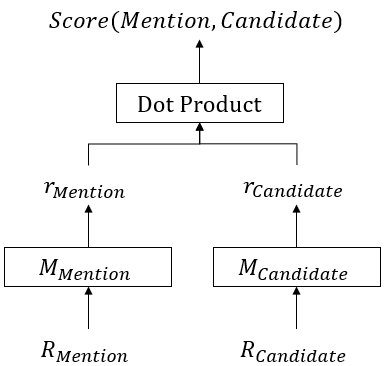
\includegraphics[scale=0.65]{BiencoderB.png}
    \hspace{1.5cm}
    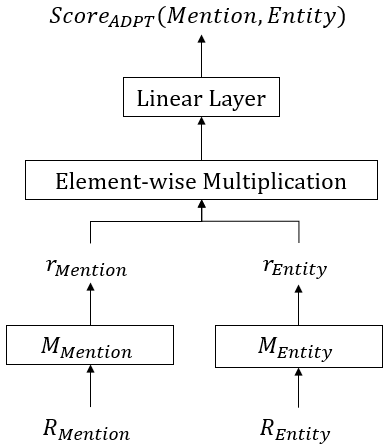
\includegraphics[scale=0.65]{BiencoderADPT.png}
    \caption{Biencoder$_{B}$ (left) and Biencoder$_{ADPT}$ (right)}
    \label{fig:biencoderB}
\end{figure}

\subsubsection{Biencoder$_{ADPT}$}
\label{sec:biencoderadaptexplanation}

Different from Biencoder$_{B}$, Biencoder$_{ADPT}$ uses a binary classification setting. For this purpose, a training set is constructed. Every mention and the corresponding correct entity are added with a positive label, and the incorrect entities for a mention are added with a negative label. Hence, the dataset $S$ has the form:

\begin{equation}
    S = \{ (m_k,e_k,l_k) \ | \ l_k \in \{0,1\} \land l_k=1 \iff link(m_k) = e_k \}.
\end{equation}

\noindent where $m_k$ is a mention, $e_k \in \mathcal{E}-\emptyset$ is an entity and $l_k$ is the binary classification label of that sample. To get the class probabilities for each mention and entity pair, an additional linear layer is used. Then, the score of a pair is defined to be the probability of the positive class:

\begin{equation}
    Score_{ADPT}(\textit{Mention},\textit{ Candidate}) = \bold{W}_{ADPT} \ (r_{Mention} \odot r_{Candidate}) [positive]
\end{equation}

\noindent where $\odot$ refers to element-wise multiplication of the vectors, and $\bold{W}_{ADPT} \in \mathcal{R}^{768x2}$ is a matrix denoting the weights of the additional linear layer\footnote{the size of the final hidden vectors of BERT$_{SC}$ is 768 as it is trained from BERT$_{BASE}$}. The binary cross-entropy loss $L_{ADPT}$ is used to train this model:

\begin{equation}
    L_{ADPT}(m_i,e_i,l_i) = - l_i \log (Score_{ADPT}(m_i,e_i)) - (1-l_i) \log (1-Score_{ADPT}(m_i,e_i)).
\end{equation}

To get incorrect (negative) entities for each mention, a different strategy is used. For the initial round of training, Neg$_{R}$ entities are sampled from the entity set for each mention randomly. Here, Neg$_{R}$ is a hyperparameter. As Neg$_{R}$ increases, the size of the dataset increases and hence the training becomes longer. Even though in-batch negatives are much faster to use, the advantage of this strategy is the possibility to show the model some entities that do not have any correct mention in the KR. Since the entity distribution of the dataset used is highly skewed (see Figure \ref{fig:entpopul}), it is inevitable that the same entities are used as the random negatives for most of the mentions when in-batch negatives are used.

As in BLINK, hard negatives are defined as the top Neg$_{H}$ entities predicted for a given mention. Different from BLINK, following \cite{googleintern}, an entity is considered to be a hard negative only if it is ranked above the correct entity. Hence, some mentions may have less hard negative samples compared to others. NIL mentions always have Neg$_{H}$ number of hard negative samples. One may argue that the entities that have a score lower than 0.5 should not be considered as a hard negative since they are predicted as the negative class, empirical results suggested that adding such entities helped. Another advantage of this setting is, since hard negatives are not added to the random negatives for loss calculation, it is possible to increase Neg$_{H}$ without the need for additional memory.

The training is done in rounds, similar to BLINK (and BiEncoder$_{B}$) and \cite{googleintern}. In each round, a new set of hard negatives and random negatives are sampled, hence the training set is updated. However, hard negatives are added starting from the second round, as initially some of the model weights are initialized randomly, such as $\bold{W}_{ADPT}$. In this work, one round may correspond to one or more epochs (see Section \ref{sec:EvalExpSetupTraining})

The number of random negatives in each round, Neg$_R$ is also a hyperparameter. In the first round of training, Neg$_R$ is set to 3 as the training time increases proportionally with Neg$_R$. In the following rounds, Neg$_R$ is selected based on the number of hard negative samples. After extracting all the hard negatives for the training set, the total number of such samples are calculated, which can be denoted as $Neg_{H}^{Sum}$. Then for each mention, $Neg_R = \lfloor Neg_{H}^{Sum}/ \text{(Number of Mentions)} \rceil$ entities are sampled randomly and added to the dataset. This way, it is aimed to have a similar proportion between random and hard negatives in the training set. The aim with this was to somehow mimic the strategy of \cite{googleintern}, who uses a multi-task learning setup with equal weights to incorporate both hard and random negatives. 

One interesting property of the setup of Biencoder$_{ADPT}$ is that for the mentions with more hard negatives, i.e. mentions that are ranked lower by the model, the training set has more hard negatives compared to random negatives. We hypothesize that the need for hard negatives are higher for these kind of mentions, as it seems that the random negatives were not enough to teach the model to make the correct decision in the first round.

In the setup for Biencoder$_{ADPT}$, it is intuitive to add NIL mentions to training. The only difference between a NIL mention and a non-NIL mention is the former not having any instance in the training set with a positive label. Also, when Biencoder$_{ADPT}$ is used as an ED system by itself, it is straightforward to detect NIL mentions. Since this is a binary classification task, if the highest scoring entity of a mention has a score lower than 0.5, it should be a NIL mention, as there are no mention-entity pairs including that mention such that the label is positive. 

The architecture of Biencoder$_{ADPT}$ is shown in Figure \ref{fig:biencoderB} (right).

\newpage
\chapter{Evaluation}
\label{sec:Evaluation}
In this work, different experiments were conducted to investigate the optimal Entity Linking (EL) approach for funding information extraction. First, BERT$_{SC}$, a BERT model that is adapted to funding text, is pretrained using the Task-Adaptive Pretraining (TAPT) strategy proposed by \cite{DontStop}. Then, different state-of-the-art Named Entity Recognition (NER) components are compared and a neural Entity Disambiguation (ED) model is developed. Lastly, the end-to-end Entity Linking performance of these approaches are investigated.

In Section \ref{sec:EvalExpSetup}, the experimental setup is presented. The dataset used and the evaluation metrics are detailed in Section \ref{sec:EvalExpSetupData} and \ref{sec:EvalExpSetupEval} respectively. The training, hyperparameters and model selection is shown in Section \ref{sec:EvalExpSetupTraining}. Lastly, the result and the analysis are shown in Sections \ref{sec:EvalResults} and \ref{sec:EvalAnalysis}.

\section{Experimental Setup}
\label{sec:EvalExpSetup}

\subsection{Data}
\label{sec:EvalExpSetupData}

The dataset for funding data extraction and the knowledge repository for ED used in this research is provided by Elsevier B.V.\footnote{\url{https://www.elsevier.com/}}. The dataset consists of a set of labelled articles annotated by humans. To create this dataset, each article is annotated by three people. First, two annotators extracted the funding information from the articles independently. Then, a third annotator harmonized the decisions of the previous two annotators, resolving the conflicts if necessary. 

For developing models and evaluating various approaches, the dataset is divided into four subsets: Training, Validation$^{1}$, Validation$^{2}$ and Test. The Training split is used to train the models. Validation$^{1}$ split is used to monitor the progress of training, while Validation$^{2}$ split is used to select the best approach for each task. The intermediate error analyses are done on the Validation$^{1}$ split. Test is used to evaluate only the Elsevier baselines and the selected approach for each task. The splits are aranged such that there is no overlap in terms of articles. Table \ref{tab:goldstats} shows the number of annotated articles contained in each split.

\begin{table}[h!]
    \centering
    \begin{tabular}{c c}
    Dataset Split  & Number of Articles  \\
        \hline
    Training &  37,484\\
    Validation$^1$ & 1,000\\
    Validation$^2$ & 4,000\\
    Test & 19,920 \\
    \end{tabular}
    \caption{Number of annotated articles in each dataset split}
    \label{tab:goldstats}
\end{table}

For the ED and EL task, the Knowledge Repository provided by Elsevier is used. This repository contains 26,892 entities of funding organizations with information such as the country of origin, type of organization and different names that the organization can be referred to with. There are also sparse amount of relations between organizations to show affiliations and hierarchies. One interesting property of the repository is that most of the entities do not exist in general-purpose knowledge repositories. Hence, it is not trivial to obtain more information from other sources.

Sometimes, organizations may change their names, or may be merged with other organizations. Hence, it is possible that one funding organization is referenced by multiple entities in the repository, which is not desirable. To prevent this, entities are grouped together based on the relations indicating such cases. This operation resulted in 25,859 entity groups. It is assumed that the entities in each group refer to the same organization, and hence can be used interchangeably. Another option could be to only keep the newest versions of the entities. However, this may cause problems with disambiguating older publications, where the authors may have used an older name variant to refer to the same organization.

The data to train and evaluate the approaches for different tasks are derived from this main dataset. However, as each task has a different nature, some preprocessing and filtering is applied when necessary. 
\newline
\newline
\textit{\textbf{Task-Adaptive Pretraining (TAPT):}} For Entity Linking in funding domain, the input text is the sentences where the authors acknowledge the funding support they had received for their research. As TAPT can be done with unlabelled data, 13 million such sentences are extracted from Scopus, where they are displayed for each article. Using the identifiers of the articles, the sentences belonging to the articles in Validation$^1$, Validation$^2$ and Test splits are removed.
\newline
\newline
\textit{\textbf{Named Entity Recognition (NER):}} As mentioned in Section \ref{sec:NERMEThod}, IOB tagging is used to train and evaluate the NER models. In the dataset used for this work, the annotations are not done in terms of tokens, but in terms of character spans of the input text. That is, each gold mention is provided using their character offsets with respect to the article text. Hence, first the input text is tokenized and the labels are assigned to tokens based on some predefined rules to tackle some edge cases that mostly correspond to annotation errors. These rules are extracted based on empirical results to maximize the correctness of the annotations. The experiments were done on a portion of the training set, and all the edge cases found were present for less than $0.5\%$ of the investigated dataset. In Appendix \ref{app:NERPrepro} you may find the details of the labelling step. 

\begin{table}[h!]
    \centering
    \begin{tabular}{ccccc}
    Dataset &  &  &\#ORG& \#GRT  \\
    Split & \#Articles & \#Sentences &Mentions&Mentions \\
    \hline
    Training   &22,720&26,132& 67,671 &45,263 \\
    Validation$^{1}$ &1,000&1,284&4,333&2,770\\
    Validation$^{2}$ &4,000&5,012&16,355 & 10,112\\
    Test & 13,851 & 15,590 &37,495&25,349\\
    \end{tabular}
    \caption{Dataset splits and statistics for NER. For each split; number of articles with at least one funding sentence, number of sentences and number of mentions are shown.}
    \label{tab:goldstatsner}
\end{table}

The NER component should extract the mentions of organizations only if they funded the corresponded research. For this purpose, the classifier developed by Elsevier is used as a preprocessing step. This classifier identifies whether a sentence contains funding information or not. As the NER component will directly work with this classifier, as a preprocessing step, the dataset splits are reduced to the sentences that are identified as positive by this classifier. The second column of Table \ref{tab:goldstatsner} shows the number of articles with at least one sentence with funding information for each dataset split, and the third column shows the total number of such sentences. Furthermore, the number of organization and grant mentions on each split can be found in the fourth and fifth columns respectively. In Figure \ref{fig:nerdatalen} you may find the distribution of number of characters for the sentences and mentions contained in the Training and Validation$^1$ splits.


\begin{figure}[h!]
    \centering
    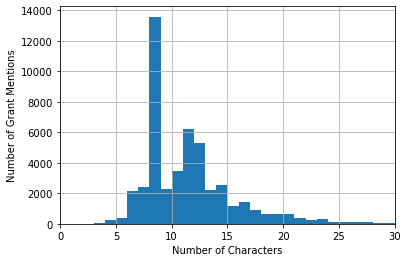
\includegraphics[scale=0.45]{grant_lens.png}
    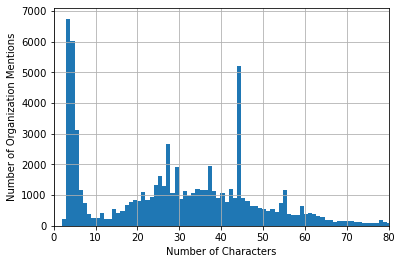
\includegraphics[scale=0.45]{org_lens.png}
    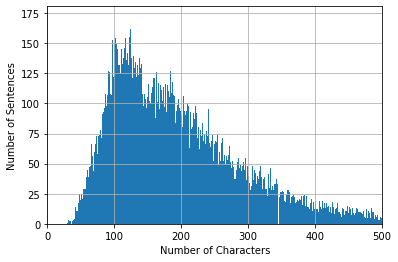
\includegraphics[scale=0.45]{sentence_lens.png}
    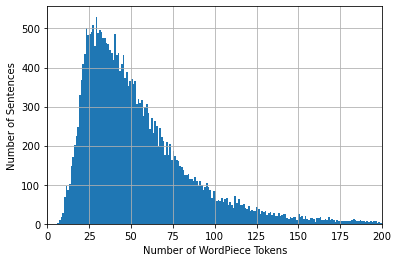
\includegraphics[scale=0.45]{sentence_tokens.png}
    \caption{Distribution of length of grant mentions (top-left), organization mentions (top-right), sentences (bottom-left) in terms of number of characters and distribution of number of tokens per sentence (bottom-right). Plots are cut over the x-axis, and the maximum x values are 75, 223, 9175 and 2760 respectively. Statistics obtained from Training and Validation$^1$ splits.}
    \label{fig:nerdatalen}
\end{figure}

\noindent \textit{\textbf{Entity Disambiguation (ED):}} For this task, the whole dataset is used. Table \ref{tab:goldstatsed} displays the statistics for each dataset split. The second column of this table shows number of articles with at least one organization mention for each split. It can be seen that not all organization mentions have a corresponding entity in the KR. These mentions will be referred to as NIL mentions. A mention being NIL means that a funding organization is extracted by the annotators, however, as this organization was not yet included in the KR, it was not linked. Because of this, all NIL mentions for this task can be classified as emerging entities (EE). These are very important for this work, as the current KR is being updated regularly consulting to the detected EEs.

\begin{table}[h!]
    \centering
    \begin{tabular}{ccccc}
    Dataset Split & \#Articles & \#ORG Mentions & \#Links & NIL Mentions  \\
    \hline
    Training & 29,118 & 95,761 & 77,972 & 18.58\% \\
    Validation$^1$ & 991 & 5,618 & 4,749 & 15.47\% \\
    Validation$^2$ & 3,943 & 19,765 & 16,689 & 15.56\% \\
    Test & 17,333 & 52,378 & 42,514 & 18.83\% \\ 
    \end{tabular}
    \caption{Dataset splits and statistics for ED. For each split, number of articles with at least one organization mention, number of organization mentions, number of mentions that are linked to an entity and the percentage of NIL mentions are shown.}
    \label{tab:goldstatsed}
\end{table}

Another interesting property of this dataset is that only the entities belonging to a small part of the KR appear as a link, as can be seen from Table \ref{tab:goldstatsed2}. For example, only 26.6\% of the entities in the KR appear as a link in the Training split. In addition, the  Validation$^1$, Validation$^2$ and Test splits contain links to entities that do not appear in the Training split. However, when  Table \ref{tab:goldstatsed3} is investigated, it is possible to see that such instances are long-tail entities. For example, even though 28.9\% of the unique entities in the Test split do not appear in the Training split; when the overall number of links are checked, only 5.14\% of the links are to these entities. Nevertheless, it is important that the ED system can link mentions of unseen entities correctly as well.


Figure \ref{fig:entpopul} shows the number of occurrences of the top 25 most frequent entities on Training and Validation$^1$ splits. It can be seen that the distribution is highly skewed, even with the most common entities. 

\begin{table}[h!]
    \centering
    \begin{tabular}{cccc}
    Dataset Split & \# Unique Entities & Overlap with Training & KR Coverage\\
    \hline
    Training & 7,234 & - & 26.9\%\\
    Validation$^1$ & 1,222 & 88.63\% & 4.54\%\\
    Validation$^2$ & 2,658 & 81.6\% & 9.88\%\\
    Test & 5,590 & 71.91\%& 20.79\%\\
    \end{tabular}
    \caption{Dataset splits and number of unique entities in each split. Third column indicates the percentage of unique entities that are also present in the Training split for Validation$^1$, Validation$^2$ and Test splits. The last column shows the percentage of Knowledge Repository covered by each split.}
    \label{tab:goldstatsed2}
\end{table}

\begin{table}[h!]
    \centering
    \begin{tabular}{ccc}
    Dataset Split & \# Links & Links not in Training\\
    \hline
    Validation$^1$ & 4,749 & 3.39\% \\
    Validation$^2$ & 16,689 & 3.52\% \\
    Test & 42,514 & 5.14\% \\
    \end{tabular}
    \caption{Dataset splits and number of links. The third column shows the percentage of links for which the target entity do not exist as a link in the Training split.}
    \label{tab:goldstatsed3}
\end{table}

\begin{figure}[H]
    \centering
    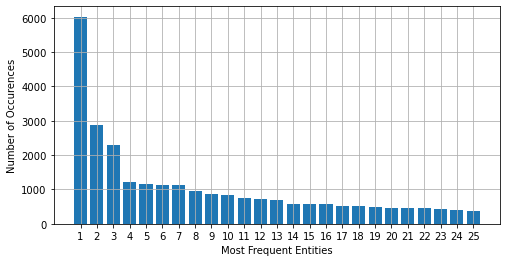
\includegraphics[scale=0.6]{ent_occ.png}
    \caption{Number of occurrences of top 25 most frequent entities. Statistics obtained using Training and Validation$^1$ splits.}
    \label{fig:entpopul}
\end{figure}


\noindent \textit{\textbf{Entity Linking (EL):}} In this work no end-to-end EL system is trained as the task of EL is tackled in two-steps, NER and ED. Hence, the data described is used to evaluate the end-to-end performance of an NER and an ED system put together. 

As the NER is also evaluated here implicitly, the Sentence classifier is used again to limit the dataset to the sentences detected by this classifier, as done for the NER task dataset. Also, all the NIL mentions are classified as emerging entities, due to the same reason reported for the ED task dataset. In fact, the dataset for EL is a subset of that of ED, limited by the sentence classifier. Tables \ref{tab:goldstatsel}, \ref{tab:goldstatsel2} and \ref{tab:goldstatsel3} show statistics of the dataset splits such as number of mentions, links and percentage of NIL mentions.

\begin{table}[H]
    \centering
    \begin{tabular}{ccccc}
     Dataset Split & \#Articles & \#ORG Mentions & \#Links & NIL Mentions  \\
     \hline
    %Validation$^1$ & 1,000  & 4,622 & 3,954  & 14.45\% \\
    Validation$^2$ & 4,000  & 16,276 & 13,958 & 14.24\% \\
    Test           & 13,851 & 37,340 & 31,153 & 16.57\% \\
    \end{tabular}
    \caption{Dataset splits and statistics for EL. For each split, number of articles with at least one organization mention, number of organization mentions, number of mentions that are linked to an entity and the percentage of NIL mentions are shown.}
    \label{tab:goldstatsel}
\end{table}


\begin{table}[H]
    \centering
    \begin{tabular}{cccc}
    Dataset Split & \# Unique Entities & Overlap with Training & KR Coverage\\
    \hline
    %Validation$^1$ & 1,034 & 89.46\% & 3.85\%\\
    Validation$^2$ & 2,302 & 83.36\% & 8.57\%\\
    Test & 4,350 & 76\%& 16.18\%\\
    \end{tabular}
    \caption{Dataset splits and number of unique entities in each split. Third column indicates the percentage of unique entities that are also present in the Training split. The entities in the Training split is determined using the dataset for the ED task. The last column shows the percentage of Knowledge Repository covered by each split.}
    \label{tab:goldstatsel2}
\end{table}

\begin{table}[H]
    \centering
    \begin{tabular}{ccc}
    Dataset Split & \# Links & Links not in Training\\
    \hline
    %Validation$^1$ & 3,954   & 3.14\% \\
    Validation$^2$ &  13,958 & 3.19\% \\
    Test &            31,153 & 4.28\% \\
    \end{tabular}
    \caption{Dataset splits and number of links. The third column shows the percentage of links for which the target entity do not exist as a link in the Training split. The entities in the Training split is determined using the dataset for the ED task.}
    \label{tab:goldstatsel3}
\end{table}

\subsection{Evaluation Metrics}
\label{sec:EvalExpSetupEval}
Each different problem tackled in this work is evaluated with a suitable metric selected from the literature.
\newline
\newline
\textit{\textbf{Task-Adaptive Pretraining (TAPT):}} To evaluate BERT$_{SC}$ and monitor its progress, Perplexity is used. This metric corresponds to the inverse probability of the dataset based on the model \cite{perplexity}, and it it is the most popular metric to evaluate language models \cite{perplexity}. 
\newline
\newline
\textit{\textbf{Named Entity Recognition (NER):}} To evaluate the Named Entity Recognition task, precision recall and F1 scores are used for each entity type, Organization and Grant. These metrics are defined in terms of True Positives (TP), False Positives (FP) and False Negatives (FN). Precision is defined as the fraction of TPs among all mentions extracted by the system, and recall is defined as the fraction TPs among all ground truth mentions. F1 score is the harmonic mean of precision and recall metrics. A mention is considered to be a TP if and only if both the extracted span and type information is correct. A FP corresponds to a mention that is extracted by the system wrongly, and a FN corresponds to a mention that is not extracted by the system while being present in the ground truth. This scheme is chosen as it is inline with evaluation of the CoNLL-2003 NER task \cite{conll}.
\newline
\newline
\textit{\textbf{Entity Linking (EL):}} To evaluate the EL task, a strategy inspired by GERBIL \cite{gerbil} is used. GERBIL is a framework for evaluating various entity-related tasks, such as NER, ED and EL. The framework supports many popular databases, hence, systems evaluating on such datasets can use it when they provide an API support. However, since this work is using a domain-specific and private dataset, it is not possible to make use of it directly. Hence, the metrics are reimplemented consulting the paper \cite{gerbil} and the GitHub repository\footnote{\url{https://github.com/dice-group/gerbil}}. 

GERBIL offers various settings to evaluate systems. In this work, ``Normal'', ``EE'' (Emerging Entities) and ``InKB'' (In Knowledge Base) settings are used for evaluation and the results for each are reported separately. 

To calculate the scores in ``Normal'' setting, for each document, the true positive (tp), false positive (fp) and false negative (fn) instances are counted. First, for each gold annotation, a matching annotation is looked for in predictions. Two annotations are considered to be matching based on strict criteria. If a match is found, this counts as a tp. Gold annotations for which no match is found are counted as fn. Similarly, the predictions that were not marked as a match for any gold annotation are counted as fp. If a prediction is marked as a match for a gold annotation, it could not be matched again. And, a gold annotation could not be matched with more than one prediction. After obtaining the tp, fp and fn counts; precision, recall and F1-score for that document are calculated. The precision, recall and F1-score for all the documents are averaged to produce macro averaged results. To obtain micro averaged results; the tp, fp and fn counts of all documents are summed together before calculating precision, recall and F1-score. Equations \ref{eq:pr}, \ref{eq:re}, \ref{eq:f1} show the calculation of scores from tp, fp and fn counts.

\begin{equation}
\label{eq:pr}
    \text{Precision} = \frac{\#tp}{\#tp+\#fp} 
\end{equation}
\begin{equation}
\label{eq:re}
    \text{Recall} = \frac{\#tp}{\#tp+\#fn} 
\end{equation}
\begin{equation}
\label{eq:f1}
    \text{F1 Score} = \frac{2\cdot\text{Precision}\cdot\text{Recall}}{\text{Precision}+\text{Recall}} 
\end{equation}

GERBIL distinguishes NIL mentions to two, emerging entities and ones where the system cannot produce a link. In this work, for the ED task, it is known that all NIL mentions are emerging entities, and the systems developed are not able to make such distinction between NIL mentions. Hence, for the EL task, the mentions extracted by the NER components are also assumed to be emerging entities, even though this may not always be the case. Based on this assumption, to get the scores for the ``EE'' setting, the tp counts are discarded when the annotations both contained an entity that is in the KR. The gold annotations that were not matched with any prediction did not count as fn if the entity was in the KR. Similarly, the predictions that were not matched did not count as fp if the entity was in the KR. For the ``InKB'' setting, the tp counts are discarded when the entities were both NIL. The gold annotations that were not matched with any prediction did not count as fn if the entity was NIL. And, the predictions that were not matched did not count as fp if the entity was NIL.
\newline
\newline
\textit{\textbf{Entity Disambiguation (ED):}} To evaluate the ED systems, the metrics introduced in \cite{NILMentions} is used. This paper has a similar ``InKB'' and ``EE'' setting with GERBIL. They do not have a ``Normal'' setting, however, they report micro and macro averaged accuracy over the whole samples. In the ``InKB'' and ``EE'' setting, the metrics used are precision, recall and F1 score. In this work, the reason why accuracy is reported in ``Normal'' setting is that, since all NIL mentions are assumed to be emerging entities, precision and recall becomes the same according to GERBIL. Different from \cite{NILMentions}, in the ``EE'' and ``InKB'' settings, micro averaged results are calculated instead of macro. 


\subsection{Training, Hyperparameters and Implementation}
\label{sec:EvalExpSetupTraining}
\todo{I thought of putting this section to 'Approach' chapter but then the evaluation metrics are not defined yet}
To conduct the experiments, first, the models introduced in Chapter \ref{chapter:Approach} are trained and implemented. For training, the Training split prepared for that specific task is used for each model. The details for all the models are explained below.
\newline
\newline
\textit{\textbf{BERT}}$_{SC}$\textit{\textbf{:}}
The weights of BERT$_{SC}$ are first initialized with the case-preserving version of BERT$_{BASE}$. Following TAPT, the model is trained end-to-end with the sentences extracted from Scopus, using Masked Language Modeling (MLM). The choice of a case-preserving model is due to the fact that case information can provide important information to the NER task, for example, it is common in English to capitalize organization names. The implementation is based on the GitHub repository of the paper where TAPT was introduced\footnote{\url{https://github.com/allenai/dont-stop-pretraining}} \cite{DontStop}. Throughout training, the progress is monitored on Validation$^1$. The hyperparameters recommended by \cite{DontStop} is used as much as possible. Number of epochs are reduced from the recommended number (100) to 2 as the training set is rather large. It is thought that 1 epoch would be sufficient, and a second epoch would be beneficial to see whether Validation$^1$ scores would improve with more epochs or not. The batch size is set to 4 due to memory requirements, but using gradient accumulation, an effective batch size of 2048 is maintained as recommended. 

However, the initial setup to train BERT$_{SC}$ could not be performed. According to the initial setup, TAPT was going to be performed for around 13,500 steps for 2 epochs. However, it was observed that after 2 days of training, only 1000 steps were finished, and hence, only around 2 million training examples were utilized. Due to the time constraints, it was determined to stop the training at that point. After 1000 steps, a perplexity of 2.8612 is achieved on the Validation$^1$ set. Figure \ref{fig:perp} shows the change of perplexity on Validation$^1$, recorded every 20 training steps. Based on this plot, we believe that it is possible to obtain a model with higher performance when the training with the full dataset is completed. However, this is left to future work.

The training of BERT$_{SC}$ is done on an NVIDIA Tesla K80 GPU with 12 GB of memory. More details on the hyperparameter configuration can be found in Appendix \ref{sec:app:bertsc}.

\begin{figure}[H]
    \centering
    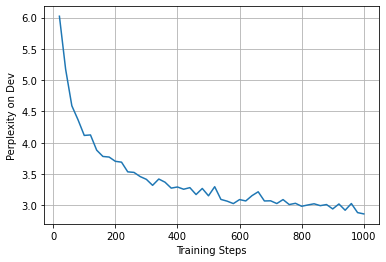
\includegraphics[scale=0.7]{perpplot.png}
    \caption{Perplexity on Validation$^1$ during training}
    \label{fig:perp}
\end{figure}

\noindent \textit{\textbf{Flair}}$^{NER}$\textit{\textbf{:}} The implementation of Flair$^{NER}$ is done using the Flair library \cite{flairlib}. In this library, both $LSTM^{forward}_{Flair}$ and $LSTM^{backward}_{Flair}$ trained on the 1 billion word corpus \cite{onebillion} are available. Using these and pretrained GloVe embeddings, the BiLSTM-CRF model is trained on the Training split and the progress is monitored on Validation$^1$ split using the training interface of Flair.  Mainly, the hyperparameters and training strategy reported in \cite{flairpaper} is followed, while changing minor things to address the computational limitations. The batch size was set to 8 and the model started training with a learning rate of 0.1. When for 2 epochs, no improvement on the Validation$^1$ split was observed, the learning rate was halved. The training is stopped when no improvement was made in a certain learning rate, amounting to 37 epochs in total. The performance on Validation$^1$ was measured as micro-averaged F1 score of the output tags. The models were saved at the end of each epoch, and the model that performed best on Validation$^1$ is selected. It was observed that the model at the end of 33 epochs was the best one. The losses, scores and learning rates per epoch are presented in Appendix \ref{sec:app:flairner}. One epoch of training Flair$^{NER}$ took approximately 50 minutes on an NVIDIA Quadro T1000 GPU with 4GB memory. 
\newline
\newline
\textit{\textbf{BERT}}$^{NER}$\textit{\textbf{:}} All parameters of BERT$^{NER}$ are fine-tuned end-to-end with different hyperparameter settings. The progress of training is monitored on Validation$^1$ across epochs, with respect to the same evaluation metric of the NER task.

Devlin et al. (2019) \cite{BERT} suggested different hyperparameter settings for fine-tuning BERT: a batch size of 16 or 32, learning rate of $5\times10^{-5}$, $3\times10^{-5}$ or $2\times10^{-5}$; and training for 2, 3 or 4 epochs. Due to memory requirements, the batch size is set to 8. Then, the model is trained for 10 epochs with a learning rate of $2\times10^{-5}$, while saving the model at the end of each epoch. On top of that, 3 more models are trained using a linear learning rate scheduler for 2, 3 and 4 epochs respectively. The number of warmup steps is set to 50. For implementation, the library Transformers \cite{huggingface} by Hugging Face\footnote{\url{https://huggingface.co/}} is used.

After the experimentation with different hyperparameter settings, it was decided that training for 3 epochs with a linear learning rate scheduler produced the best results. Appendix \ref{sec:app:bertner} shows detailed results on this experimentation.

BERT$^{NER}$ can process a maximum of 512 tokens per input, similar to BERT$_{BASE}$. Hence, the sentences having more tokens are split into smaller chunks, such that there is no overlap between chunks and no word is scattered across chunks. Later on, the predictions are merged as a postprocessing step. The training is done using an NVIDIA Tesla K80 GPU with 12 GB of memory. On this device, one epoch took approximately 1 hour. 
\newline
\newline
\textit{\textbf{BERT}}$^{NER}_{SC}$\textit{\textbf{:}} BERT$^{NER}_{SC}$ is trained with the exact same hyperparameter settings that produced the best results for BERT$^{NER}$, i.e. for 3 epochs with a linear learning rate scheduler.

One aim of this study is also showing the effect of domain adaptation. This will be done by comparing BERT$^{NER}$ and BERT$^{NER}_{SC}$. To be able to show that the improvement gained by pretraining is not random, a second BERT$^{NER}_{SC}$ is trained with the second-best hyperparameter setting, for 2 epochs with a linear learning rate scheduler. However, the aim of this second BERT$^{NER}_{SC}$ is just for observing the effect of domain adaptation, not for measuring the success of any other task. Hence, when BERT$^{NER}_{SC}$ is referred to in any other setting, it is the one trained for 3 epochs.

BERT$^{NER}_{SC}$ can also process a maximum of 512 tokens, and is also trained on the same GPU with BERT$^{NER}$. One epoch of training took approximately 1 hour.
\newline
\newline
\textit{\textbf{Biencoder}}$_{B}$\textit{\textbf{:}} The implementation of Biencoder$_{B}$ was inspired by its GitHub repository\footnote{\url{https://github.com/facebookresearch/BLINK/tree/master/blink}}. Mainly, the code for data preprocessing was obtained from this repository. The models and training was implemented using PyTorch \cite{pytorch} and Transformers library by Hugging Face.

As there was no computational power to be able to do an extensive hyperparameter search, the values reported by \cite{scalablezeroshot} is followed as much as possible. In BLINK, the maximum number of tokens for the mention representation ($R_{Mention}$) are either 32 or 128, depending on the dataset. This number is set to 64 in this work. Originally it was planned to set it to 32 to address the memory limitations, however, it was observed that there were mentions longer than 32 tokens themselves.

For candidate representation ($R_{Candidate}$), BLINK uses 128 tokens. However, in this setting, there are candidates that have longer representations. To be more specific, there are 96 entities with representation longer than 128 tokens, 36 entities longer than 256 tokens, and 23 entities longer than 256. Hence, for the 96 entities that had longer representations, a label is removed iteratively until the representation was equal to or shorter than 128 tokens. The label that had the highest sorted Levenshtein distance with any other label is removed in each iteration, as it was thought that this label would be the least informative.

BLINK uses a batch size of 128, and adds 10 hard negatives (Neg$_H$=10) among these in-batch negatives. Hence, for a mention, they make use of a maximum of 127 random negatives and a maximum of 137 negatives in total ($max(|IE|)=127+10=137$). As the training is done on a GPU with 12 GB memory, this batch size could not be maintained in terms of random negatives. Hence, the hyperparameters are scaled down proportionally. It was observed that a maximum batch size of 16 was possible. Proportionally, Neg$_H$ is set to 1, making $max(|IE|)=15+1=16$.

Even though a batch size of 128 cannot be maintained in terms of in-batch random negatives, it is possible to maintain this number in terms of gradient updating using gradient accumulation. Initially, the batch size was set to be inline with BLINK. Similarly, the learning rate was set to $10^{-5}$. However, no learning was observed with this setting. We hypothesize that it is because of the size of the dataset. At the end, the batch size was set to 64 using gradient accumulation and the learning rate was set to $2 \times 10^{-5}$, which is also the minimum learning rate recommended by \cite{BERT}.

The models in BLINK are trained for either 4 or 5 epochs. It is not clear whether the hard negative sampling is done for each epoch or not. However, as they report that they are following the strategy of \cite{googleintern}, it will be assumed that one epoch corresponds to one round for this case. Based on this, initially, it was thought to have 4 rounds of training, each consisting of 1 epoch. No hard negatives are added in the first round, as some weights of the model are initialized randomly anyway. To observe the course of training and the change in performance after each round, Validation$^1$ is used.

Table \ref{tab:biencoderbres} shows the performance of Biencoder$_B$ on Training and Validation$^1$ sets after the first two rounds. It can be seen that after the second round, the performance drops further for the InKB setting but improves for the EE setting, resulting in an overall performance decline as shown with accuracy. We hypothesize that the second round of training resulted in better separation of the scores of NIL and not-NIL mentions, however, did not improve the model in terms of finding the correct entity. 


\begin{table}[H]
    \centering
    \begin{tabular}{cccc}
    &&Micro-Averaged & Macro-Averaged\\
    Round    & Dataset & Accuracy &Accuracy \\
    \hline
    1  & Training & 61.88&62.9\\
    2  & Training & 59.2&	59.21\\
    1  & Validation$^1$ & 60.16	&64.04\\
    2  & Validation$^1$ & 55.06	&59.13\\
    \end{tabular}
    
    \vspace{0.5cm}\begin{tabular}{ccccc}
    &&&EE Setting & \\
    Round    & Dataset & Precision & Recall & F1-Score \\
    \hline
    1  & Training &60.32&	60.64&	60.48 \\
    2  & Training &64.42&	85.03&	73.3 \\
    1  & Validation$^1$ &50.4&	57.31&	53.63 \\
    2  & Validation$^1$ &54.1&	72.96&	62.13\\
    \end{tabular}
    
    \vspace{0.5cm}\begin{tabular}{ccccc}
    &&&InKB Setting & \\
    Round    & Dataset & Precision & Recall & F1-Score \\
    \hline
    1  & Training &62.24&62.16	&62.2\\
    2  & Training &57.51&53.31	&55.33\\
    1  & Validation$^1$ &62.25&60.69	&61.46 \\
    2  & Validation$^1$ &55.31&51.78	&53.49\\
    \end{tabular}
    
    \caption{Scores of Biencoder$_B$ for the first two rounds. A threshold of 0.324 is used for the first and 0.321 for the second round.}
    \label{tab:biencoderbres}
\end{table}

To see the separation between NIL-mentions and non-NIL mentions, it is possible to model the distribution of scores. For this purpose, two normal distributions are fit on the normalized scores (see Section \ref{sec:biencoderbexplanation} for details of the normalization) of the highest ranked entity for each mention, one for NIL-mentions and one for others. The parameters of the distribution are calculated using Maximum Likelihood and Validation$^1$ dataset, and are shown in Table \ref{tab:nilnotnilBparams}. Figure \ref{fig:biencoderbnil} shows the histogram of scores for each distribution. When the Bhattacharyya distance  \cite{bhatt} is checked, it is possible to see that the distribution of NIL-mention scores are more different than the other mentions in Round 2, compared to Round 1. The choice of this metric is due to the fact that it is reported as a convenient metric to measure the class separability of normal distributions \cite{bhatt}.

\begin{table}[H]
    \centering
    \begin{tabular}{c|cc|cc|c}
    & \multicolumn{2}{c|}{NIL Mentions} & \multicolumn{2}{c|}{Other Mentions} & Bhattacharyya\\
     Round  &  Mean & Std. Dev. &  Mean &  Std. Dev.& Distance\\
     \hline
    1     &  0.311& 0.109&0.465&0.11&0.247\\ 
    2     & 0.263&0.099 & 0.534 & 0.17&0.541\\
    \end{tabular}
    \caption{Parameters of the distributions for scores and the Bhattacharyya distance between the two distributions for each round.}
    \label{tab:nilnotnilBparams}
\end{table}

\begin{figure}[H]
    \centering
    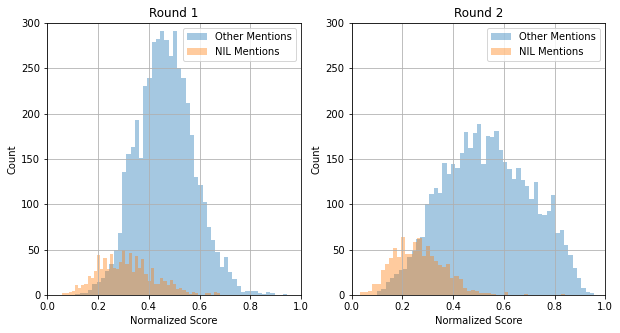
\includegraphics[scale=0.5]{biencoderbnil.png}
    \caption{Distribution of scores for Biencoder$_B$, first two rounds, on Validation$^1$.}
    \label{fig:biencoderbnil}
\end{figure}

Based on the results, the training of Biencoder$_B$ is stopped after two rounds, and was not used any further. The training of the first round took 1.3 and the second round took 1.7 hours in the NVIDIA Tesla K80 GPU with 12 GB of memory.
\newline
\newline
\textit{\textbf{Biencoder}}$_{ADPT}$\textit{\textbf{:}} To train Biencoder$_{ADPT}$, the same batch size and learning rate with that of Biencoder$_{B}$ is used. The progress of the training is also monitored using the Validation$^1$ split. 

The model is trained for 4 rounds, each consisting of one epoch. The initial round of training is done just with random negatives, and Neg$_R$ is set to 3. This hyperparameter is not tuned as there is not much performance improvement expected from the initial round. It could be that a higher Neg$_R$ leads to a better result, however, the training time would also increase accordingly. In the following rounds, Neg$_H$ is set to 10, as BLINK also uses 10 hard negatives. Based on the formula introduced in Section \ref{sec:biencoderadaptexplanation}, Neg$_R$ is set to 3, 2 and 2 for the second, third and fourth rounds respectively. Also, in the initial round, class weights are used for loss calculation to prevent the model to predict everything as the negative class. According to the random negative sampling strategy, a weight of 0.25 is given to the negative class and 0.75 is given to the positive class. However, class weights are not used in the following rounds, even though the class imbalance continues. During training, it was seen that not using class weights was slightly better for the performance. This could be because in these rounds the negative samples are selected with hard negative mining, and hence are very informative.

Table \ref{tab:hardnegsbiencoder1} (upper) shows the number of hard negatives for Training and Validation$^1$ splits after each round. As can be seen, the mentions with no hard negatives increase significantly after the second round, and this increase becomes much smaller in the following rounds. In this setting, the training took around 5, 8.5, 6.5 and 6.5 hours for the first, second, third and fourth rounds respectively; using the NVIDIA Tesla K80 GPU with 12 GB of memory.

\begin{table}
    \centering
    \hspace*{-1.2cm}\begin{tabular}{ccccccccccccc}
    Dataset  & Round & None & 1 & 2 & 3 & 4 & 5 & 6 & 7 & 8 & 9 & 10+ \\
    \hline
    Training & 1 & 51,482&12,711&4,470&1,873&1,244&1,034&691	&517&	450&356&3,144\\
    Training & 2 & 70,566&3,024	&916&	516	&327	&194&	147&	135	&133&	104&1,910\\
    Training & 3 & 71,547&3,329	&899&	402	&272	&187&	153&	102&	88&	85&908\\
    Training & 4 & 73,273&2,273	&821&	313	&200	&117&	85	&57	&62&	53&718\\
    \hline
    Validation$^1$ & 1 & 3,063&771&283&	122&63	&63	&49&	36	&17&	30&252\\
    Validation$^1$ & 2 &4,204&173&58	&36&24&	6	&12&	12	&12&	5 &207\\
    Validation$^1$ & 3 & 4,222&212&74&	33&19	&10	&14&	12&	9&	5&139\\
    Validation$^1$ & 4 & 4,291&148&64&	24&13	&12	&13&	5&	9&	10 &160\\
    \end{tabular}
    
    \vspace*{0.5cm}\hspace*{-1cm}\begin{tabular}{ccccccccccccc}
    Dataset  & Round & None & 1 & 2 & 3 & 4 & 5 & 6 & 7 & 8 & 9 & 10+ \\
    \hline
    Training & 1 & 59,711&9,356&2,787&1,559&907&794&436&326&263&205&1,628\\
    Training & 2 & 73,259&2,562&579&374&180&115&100&66&48&42&647\\
    Training & 3 & 74,484&2,141&484&252&152&79&68&45&33&17&217\\
    Training & 4 & 75,403&1,875&295&107&60&38&31&17&9&14&123\\
    \hline
    Validation$^1$ & 1 & 3,574&556&161&99&49&57&20&25&15&14&179\\
    Validation$^1$ & 2 &4,288&183&43&31&12&12&11&10&5&3&151\\
    Validation$^1$ & 3 &4,355&159&51&32&14&20&12&8&4&6&88\\
    Validation$^1$ & 4 &4,354&178&37&13&7&11&11&8&6&3&121 \\
    \end{tabular}
    
    \caption{Number of not-NIL mentions with \{None, 1,2,...,9 ,10 or more\} hard negatives in each round for Biencoder$_{ADPT}$. Upper table is with the \textbf{first} set of hyperparameters, and lower table is with the \textbf{second} set of hyperparameters.}
    \label{tab:hardnegsbiencoder1}
\end{table}


As a second set of hyperparameters, it was tried to train each round for 2 epochs instead of one. Also, the maximum tokens for $R_{Candidate}$ is set to 256. It was thought that a longer representation would be better in the event that new entities would have many labels. The number was not increased to 512, in case the Cross-Encoder of BLINK \cite{scalablezeroshot} would be implemented later on. A separate experiment to see the effect of this increase to the performance was not conducted as the impacted entities cover 2.42 \% of Training, 2.3 \% of Validation$^1$, 2.41 \% of Validation$^2$ and 2.66 \% of Test split for the ED task. There were 1037 samples in Validation$^2$ split for which Biencoder$_{ADPT}$ made a mistake when trained with the first hyperparameter configuration, but got the correct answer when trained with the second hyperparameter configuration. Among these samples, in only 10 of them, the correct entity was affected by this change. Lastly, as the entity embeddings are precomputed before inference, this increase does not have any impact on the efficiency.

Apart from number of epochs per round and the maximum tokens for $R_{Candidate}$, the other hyperparameters were not changed. During training, following the formula, Neg$_R$ is set to 2 for second, third and fourth rounds. In this setting, the training took around 11, 15, 13.5 and 14 hours for the first, second, third and fourth rounds respectively; using the NVIDIA Tesla K80 GPU with 12 GB of memory.

\begin{table}[H]
    \centering
    \begin{tabular}{cccc}
    &&Micro-Averaged & Macro-Averaged\\
    Setting & Threshold     & Accuracy &Accuracy \\
    \hline
    1  & 0.5&83.85&87.3\\
    2  & 0.5&86.95&89.9\\
    1  & 0.732&86.61&89.17\\
    2  & 0.728&88.44&90.75\\
    \end{tabular}
    
    \vspace{0.5cm}\begin{tabular}{ccccc}
    &&&EE Setting & \\
    Setting    & Threshold & Precision & Recall & F1-Score \\
    \hline
    1  & 0.5&81.06	&47.85&	60.18\\
    2  & 0.5&84.22&	58.97&	69.37\\
    1  & 0.732&70.38&	76.24&	73.19\\
    2  & 0.728&75.75&	76.27&	76.01\\
    \end{tabular}
    
    \vspace{0.5cm}\begin{tabular}{ccccc}
    &&&InKB Setting & \\
    Setting    & Threshold& Precision & Recall & F1-Score \\
    \hline
    1  & 0.5&84.13&	90.48&	87.19\\
    2  & 0.5&87.29&	92.11&	89.64\\
    1  & 0.732&89.9&	88.53&	89.21\\
    2  &0.728&90.8&	90.68&	90.74\\
    \end{tabular}
    \caption{Comparing the two hyperparameter settings on Validation$^2$ split.}
    \label{tab:biencoderadaptres}
\end{table}

Table \ref{tab:hardnegsbiencoder1} (lower) shows the number of hard negatives for the second configuration and Table \ref{tab:biencoderadaptres} shows the results on Validation$^2$ for both hyperparameter settings. Even though a score of 0.5 is a natural threshold for NIL mention detection as the problem is cast as binary classification, a threshold that maximizes the micro averaged accuracy is selected on the Training split using grid search in the interval [0.5,1] with a step size of 0.001. 

It is possible to see that there are more mentions with no hard negatives in general for the second set of hyperparameters. Moreover, all the scores are higher on Validation$^2$ when the second hyperparameters are used. That is why, it was decided to use the model that is trained for 2 epochs per round and that has a maximum $R_{Candidate}$ of 256.

An interesting observation is, a threshold selection is beneficial for NIL mention detection, which is shown by the EE evaluation setting. This could indicate that the models do not have a full capability of detecting NIL mentions themselves. 

Appendix \ref{sec:app:biencoderadapt} presents more results on Training and Validation$^1$ splits for each round of training.

\section{Results}
\label{sec:EvalResults}
The results for NER, ED and EL are presented in this section. Different approaches are compared on the Validation$^2$ splits, and the best performing appraoch is compared with Elsevier's baseline in that task on the Test split.
\newline
\newline
\textit{\textbf{Named Entity Recognition (NER) and Task-Adaptive Pretraining (TAPT):}}
To compare the developed NER models, the current NER component of Elsevier, which is based on Stanford NER \cite{stanfordNER},  is used as a baseline.

\begin{table}
    \centering
    \begin{tabular}{c| c c c| c c c}
    &\multicolumn{3}{c|}{Organization}&\multicolumn{3}{c}{Grant} \\
    System&Precision&Recall&F1&Precision&Recall&F1\\
    \hline
    Els. Baseline & 73.7&	75.1&74.39&94.11&94.77&94.44
 \\[0.7ex]
    BERT$^{NER}$ & 79.18&86.03&82.46&94.71&97.39&96.03
\\[0.7ex]
    BERT$^{NER}_{SC}$ & 80.28&86.54&83.29&94.9	&97.63&96.24
  \\[0.7ex]
    Flair$^{NER}$& 85.83&78.02&81.74&97.56&95.24&96.39
 \\[0.7ex]
    \end{tabular}
    \caption{NER Results on Validation$^2$ split}
    \label{tab:all_ner_results}
\end{table}

Table \ref{tab:all_ner_results} compares the precision, recall and F1 scores for Organization and Grant mentions on Validation$^2$ dataset. It can be seen that all models perform well on extracting grant mentions, while Flair$^{NER}$ obtains the highest F1 score with a small difference. In contrast, using neural language models improve the performance on Organization mentions with a large margin, resulting in a minimum absolute increase of 7.4 points in terms of F1.

BERT$^{NER}$ sligtly outperforms Flair$^{NER}$ in terms of Organization F1-score by an increase of 0.7 points. However, the main difference is the precision and recall values. Flair$^{NER}$ achieves a precision that is 6.6 points higher than that of BERT$^{NER}$, while BERT$^{NER}$ achieves a recall that is 8 points higher. In funding data extraction, for NER component, a higher recall is preferred in this study as if a mention is missed completely, there is nothing that can be done about it.

BERT$^{NER}_{SC}$ improves upon BERT$^{NER}$ further, showing the importance of domain adaptation. When trained with the exact same setup, it is possible to see an improvement of 1 points in precision and 0.5 points in recall. To show that this was not a coincidence, Table \ref{tab:bertsccompareother} shows the performance of BERT$^{NER}$ and BERT$^{NER}_{SC}$ trained for 2 epochs with a learning rate scheduler on the Validation$^2$ split. It can be seen that domain adaptation improves the performance on this hyperparameter setting as well.

\begin{table}
    \centering
    \begin{tabular}{c| c c c| c c c}
    &\multicolumn{3}{c|}{Organization}&\multicolumn{3}{c}{Grant} \\
    System&Precision&Recall&F1&Precision&Recall&F1\\
    \hline
    BERT$^{NER}$ (2 epochs) &  78.44&85.8&81.96&94.59&97.43&95.99
 \\[0.7ex]
    BERT$^{NER}_{SC}$ (2 epochs) &  79.54&86.56&82.9&94.73&97.55&96.12
  \\[0.7ex]
    \end{tabular}
    \caption{Comparison of BERT$^{NER}$ and BERT$^{NER}_{SC}$ with the second-best hyperparameter setting, i.e. 2 epochs with a learning rate scheduler.}
    \label{tab:bertsccompareother}
\end{table}

\begin{table}
    \centering
    \begin{tabular}{c| c c c| c c c}
    &\multicolumn{3}{c|}{Organization}&\multicolumn{3}{c}{Grant} \\
    System&Precision&Recall&F1&Precision&Recall&F1\\
    \hline
    Els. Baseline &  76.17 & 72.87  & 74.48 & 93.37   & 93.24  & 93.31
 \\[0.7ex]
    BERT$^{NER}_{SC}$ &  79.08 & 85.31 & 82.08& 93.95&   96.54&   95.23
  \\[0.7ex]
    \end{tabular}
    \caption{NER Results on Test split}
    \label{tab:all_ner_results_test}
\end{table}

At the end, it is decided to use BERT$^{NER}_{SC}$ as the NER component to extract mentions of funding bodies. Table \ref{tab:all_ner_results_test} compares the results of BERT$^{NER}_{SC}$ and Elsevier Baseline on the Test split. It is possible to see that the performance gain persists on the Test split as well. Hence, it is concluded that this work improved upon Elsevier's NER baseline by 2.9 points gain in precision, 12.4 points gain in recall and 7.6 points gain in F1 score.
\newline
\newline
\noindent \textit{\textbf{Entity Disambiguation (ED):}} Table \ref{tab:edresultsval} shows the performance of the ED systems on Validation$^2$. Biencoder$_{ADPT}$ is the one that is trained with the best hyperparameters setting. The performance of Biencoder$_{ADPT}$ with a 0.5 threshold for NIL mention detection is reported, as this is the natural one given that ED is cast as binary classification. Also, another threshold that maximizes the micro averaged accuracy on Training split is selected by applying grid search in the interval [0.5,1] with a step size of 0.001. 

As a baseline, the ED system that is developed by Elsevier is used. On top of that, the performance of a system that is solely based on Commonness is reported. Commonness measures the maximum likelihood probability of an entity being the link to the given mention \cite{balog}. For a mention-entity pair, it is calculated as number of times that the mention was linked to the given entity, divided by the number of times that the mention appears as a link \cite{balog}. For this system, the commonness values are obtained using the Training split, and the mention is linked to the entity with which it has the highest commonness value. If a mention did not appear as a link in the Training split (and hence no commonness value is recorded), it is linked to NIL.

The results show that a threshold that is higher than 0.5 helps improving the performance of Biencoder$_{ADPT}$. However, even with this threshold, Elsevier's model outperforms Biencoder$_{ADPT}$ significantly. Also, even though it is highly simple, the Commonness baseline has surprisingly good results.

\begin{table}
    \centering
    \begin{tabular}{cccc}
    &&Micro-Averaged & Macro-Averaged\\
    System    & Threshold & Accuracy &Accuracy \\
    \hline
    Biencoder$_{ADPT}$  & 0.5 & 86.95&89.9\\
    Biencoder$_{ADPT}$  & 0.728 & 88.44&90.75\\
    Commonness  & -  &83.8&85.81 \\
    Elsevier Baseline & - & 91.02&92.84\\
    \end{tabular}
    
    \vspace{0.5cm}\begin{tabular}{ccccc}
    &&&EE Setting & \\
    System    & Threshold & Precision & Recall & F1-Score \\
    \hline
    Biencoder$_{ADPT}$  & 0.5 & 84.22& 58.97&	69.37\\
    Biencoder$_{ADPT}$  & 0.728 & 75.75& 76.27&	76.01\\
    Commonness  & -  &53.55& 88.2&	66.64 \\
    Elsevier Baseline & - &79.11& 78.67&	78.89 \\
    \end{tabular}
    
    \vspace{0.5cm}\begin{tabular}{ccccc}
    &&&InKB Setting & \\
    System    & Threshold & Precision & Recall & F1-Score \\
    \hline
    Biencoder$_{ADPT}$  & 0.5 & 87.29&92.11&89.64\\
    Biencoder$_{ADPT}$  & 0.728 & 90.8&90.68&	90.74\\
    Commonness  & - &94.22&82.99	&88.25 \\
    Elsevier Baseline & - & 93.2&93.29&	93.25\\
    \end{tabular}
    
    \caption{Performance comparison of different ED models on the Validation$^2$ split.}
    \label{tab:edresultsval}
\end{table}

\begin{table}
    \centering
    \begin{tabular}{cccc}
    &&Micro-Averaged & Macro-Averaged\\
    System    & Threshold & Accuracy &Accuracy \\
    \hline
    Best  & ? & \\
    Elsevier Baseline & - & 90.26&	90.84\\
    \end{tabular}
    
    \vspace{0.5cm}\begin{tabular}{ccccc}
    &&&EE Setting & \\
    System    & Threshold & Precision & Recall & F1-Score \\
    \hline
    Best  & ? & \\
    Elsevier Baseline & - & 80.03&	81.49&	80.75\\
    \end{tabular}
    
    \vspace{0.5cm}\begin{tabular}{ccccc}
    &&&InKB Setting & \\
    System    & Threshold & Precision & Recall & F1-Score \\
    \hline
    Best  & ? & \\
    Elsevier Baseline & - & 92.69&	92.3&	92.5\\
    \end{tabular}
    		

    \caption{Performance comparison of the best ED model developed and Elsevier baseline on Test split.}
    \label{tab:edresultstest}
\end{table}
Table \ref{tab:edresultstest} compares the performance of the best performing model (...) and the Elsevier baseline on Test split.\todo{after ED model selection}
\newline
\newline
\noindent \textit{\textbf{Entity Linking (EL):}} Table \ref{tab:elresultsvalid} shows the end-to-end EL performance of different NER and ED systems combined. It can be seen that, in all settings, the performance is lower when the NER of Elsevier is used. It was on shown on Table \ref{tab:all_ner_results} that BERT$_{SC}^{NER}$ improves upon Elsevier baseline by 6.6 ,11.44 and 8.9 points in terms of precision, recall and F1 score of Organization mentions, on Validation$^2$ split. Table \ref{tab:elresultsvalid} shows that the EL performance of ED models have a similar performance increase in the ``Normal'' setting when BERT$_{SC}^{NER}$ is used for NER instead of Elsevier baseline. 

It can also be seen that the InKB performance is significantly higher than the performance on EEs. Hence, it can be hypothesized that improving NIL mention detection is something that should be worked on. In addition, in the InKB setting, the recall values are lower than precision, but this does not hold for the Normal setting. This may be caused by the sub-optimal NIL mention detection threshold as well, failing to generate the link to the correct entity when the assigned score is lower than the linear threshold.

\begin{table}
    \centering
    \begin{tabular}{c|cccc}
    &  Mean & Std. & Min. & Max.\\
    \hline
    Sentence Length (in characters) &  229 & 126 & 65 & 919\\
    Sentence Length (in WordPiece tokens) & 63 & 37 & 19 & 257\\
    Number of ORG mentions per sentence & 3 & 2 & 0 & 10\\
    \end{tabular}
    \caption{Statistics of the subsample for the runtime experiment.}
    \label{tab:efficiencystats}
\end{table}

\begin{table}
    \centering
    \begin{tabular}{c|cc}
    System   & With GPU & Without GPU  \\
    \hline
    BERT$_{SC}^{NER}$  & $2.55 \pm 0.14$ & $16.61 \pm 1.58$\\
    ?  & \\
    \end{tabular}
    \caption{Mean and standard deviation runtime (in seconds) for 100 sentences and 306 ORG mentions, measured with and without GPU.}
    \label{tab:efficiencyresults}
\end{table}

\begin{table}
    \centering
    \begin{tabular}{c c c c c| c c c}
    \multicolumn{2}{l}{(``Normal'' Setting)}&\multicolumn{3}{c|}{Micro-Averaged}&\multicolumn{3}{c}{Macro-Averaged} \\
    NER & ED &Precision&Recall&F1&Precision&Recall&F1\\
    \hline
    Els. Baseline & Commonness & 63.41&64.96&64.18&72.45&70.14&	70.31\\
    Els. Baseline & Els. Baseline & 67.92&69.57&68.74&76.74&74.28&	74.44\\
    Els. Baseline & Biencoder$_{ADPT}$ &66.58&68.2&67.38&75.73&73.3&	73.46\\
    BERT$_{SC}^{NER}$ & Commonness & 69.48&75.26&72.25&75.82&78.3&	76.38\\
    BERT$_{SC}^{NER}$ & Els. Baseline & 74.19&80.36&77.15&80.17&82.88&	80.79\\
    BERT$_{SC}^{NER}$ & Biencoder$_{ADPT}$ &72.49&78.52&75.38&78.91&81.5&	79.5\\
    \end{tabular}
    
    \vspace{0.5cm}\begin{tabular}{c c c c c| c c c}
    \multicolumn{2}{l}{(``EE'' Setting)}&\multicolumn{3}{c|}{Micro-Averaged}&\multicolumn{3}{c}{Macro-Averaged} \\
    NER & ED &Precision&Recall&F1&Precision&Recall&F1\\
    \hline
    Els. Baseline & Commonness & 38.45&	45.82&41.81&	57.82&58.88&	57.78\\
    Els. Baseline & Els. Baseline &51.52&	41.54&46	 & 71.29&70.34  & 70.32 \\
    Els. Baseline & Biencoder$_{ADPT}$ &50.36&	39.47&44.26&	70.87&70.19&	70.09\\
    BERT$_{SC}^{NER}$ & Commonness & 45.67&	58.5&51.3&	62.43&64.48&	62.84\\
    BERT$_{SC}^{NER}$ & Els. Baseline &56.07&	53.8&54.91&	73.38&73.53&	72.97 \\
    BERT$_{SC}^{NER}$ & Biencoder$_{ADPT}$ &56.6&	49.78&52.97&	74.39&74.26&	73.85\\
    \end{tabular}
    
    \vspace{0.5cm}\begin{tabular}{c c c c c| c c c}
    \multicolumn{2}{l}{(``InKB'' Setting)}&\multicolumn{3}{c|}{Micro-Averaged}&\multicolumn{3}{c}{Macro-Averaged} \\
    NER & ED &Precision&Recall&F1&Precision&Recall&F1\\
    \hline
    Els. Baseline & Commonness & 89.87	&68.14&	77.51&	85.1	&72.47&	76.41\\
    Els. Baseline & Els. Baseline & 87.16	&74.23&	80.17	&83.38	&77.86&	79.3\\
    Els. Baseline & Biencoder$_{ADPT}$ &86.36	&72.98&	79.11&	82.5	&76.88&	78.37\\
    BERT$_{SC}^{NER}$ & Commonness & 90.62	&78.04&	83.86	&87.69	&80.26&	82.5\\
    BERT$_{SC}^{NER}$ & Els. Baseline & 89.31	&84.77&	86.98	&86.99	&86.06&	85.72\\
    BERT$_{SC}^{NER}$ & Biencoder$_{ADPT}$ &88.24	&83.29&	85.7	&85.52	&84.79&	84.37\\
    \end{tabular}
    \caption{EL performance of different NER-ED model pairs on the Validation$^2$ split. NIL detection for Biencoder$_{ADPT}$ performed with the threshold 0.728.}
    \label{tab:elresultsvalid}
\end{table}


\begin{table}
    \centering
    \begin{tabular}{c c c c c| c c c}
    \multicolumn{2}{l}{(``Normal'' Setting)}&\multicolumn{3}{c|}{Micro-Averaged}&\multicolumn{3}{c}{Macro-Averaged} \\
    NER & ED &Precision&Recall&F1&Precision&Recall&F1\\
    \hline
    Els. Baseline & Els. Baseline & 69.83	&67.09&	68.43&	71.62&	69.24&	69.34
\\
    BERT$_{SC}^{NER}$ & ? & \\
    \end{tabular}
    
    \vspace{0.5cm}\begin{tabular}{c c c c c| c c c}
    \multicolumn{2}{l}{(``EE'' Setting)}&\multicolumn{3}{c|}{Micro-Averaged}&\multicolumn{3}{c}{Macro-Averaged} \\
    NER & ED &Precision&Recall&F1&Precision&Recall&F1\\
    \hline
    Els. Baseline & Els. Baseline & 45.93&	1.02&	43.34&	71.77&	71.07	&71.01
\\
    BERT$_{SC}^{NER}$ & ? & \\
    \end{tabular}
    
    \vspace{0.5cm}\begin{tabular}{c c c c c| c c c}
    \multicolumn{2}{l}{(``InKB'' Setting)}&\multicolumn{3}{c|}{Micro-Averaged}&\multicolumn{3}{c}{Macro-Averaged} \\
    NER & ED &Precision&Recall&F1&Precision&Recall&F1\\
    \hline
    Els. Baseline & Els. Baseline & 83.15&	72.26&	77.33&	78.05&	73.69&	74.73
\\
    BERT$_{SC}^{NER}$ & ? & \\
    \end{tabular}
    \caption{Comparison of EL performance of the best NER and ED models and the Elsevier baselines on the Test split.}
    \label{tab:elresultstest}
\end{table}


Table \ref{tab:elresultstest} compares the performance of the best performing model (...) and the Elsevier baseline on Test split. \todo{after ED model selection}
\newline
\newline
\noindent \textbf{\textit{Efficiency:}} The runtime of the best developed NER and ED component, BERT$_{SC}^{NER}$ and \textcolor{red}{X}, is measured on a random sample of 100 sentences from the Validation$^1$ split. First, BERT$_{SC}^{NER}$ is executed on the input to detect the mentions. Then, \textcolor{red}{X} is executed on the detected Organization mentions (306 in total) to perform disambiguation. Table \ref{tab:efficiencystats} shows some statistics of this subsample.

The experiment is repeated 10 times on a laptop that has an Intel Xeon E-2276M (2.80GHz, 32GB RAM) CPU and an NVIDIA Quadro T1000 GPU with 4GB memory. The average and standard deviation runtime calculated from this experiment are shown in Table \ref{tab:efficiencyresults}. \todo{after ED model selection}
    

\newpage
\section{Analysis}
\label{sec:EvalAnalysis}
%"What do these results mean (according to the objectives you have set)? Can you identify success and failure cases? Clear take-home messages."

The results obtained after the experiments give important insights on using the systems that work well in general domain for funding domain. 

\subsubsection{Task-Adaptive Pretraining}
Following the advice of the recent literature \textcolor{red}{\cite{}}, it was decided to perform domain adaptation on BERT$_{BASE}$, producing BERT$_{SC}$. For this purpose, the Task-Adaptive Pretraining (TAPT) strategy proposed by \cite{DontStop} is used. 


\begin{itemize}
    \item At the end of training, a perplexity of 2.86 is achieved on Validation$^1$, which is lower than that of BERT$_{BASE}$ reported on its held-out set \cite{BERT}.
    \item Based on the perplexity plot on Validation$^1$ shown in Figure \ref{fig:perp}, we hypothesize that it is possible to see further improvement when the training proceeds.
    \item To show the effectiveness of pretraining, two sets of BERT$^{NER}_{SC}$ models are trained, one with the best and one with the second-best hyperparameter combination observed on BERT$^{NER}$. \begin{itemize}
        \item For the best hyperparameter setting, Table \ref{tab:all_ner_results} shows that BERT$^{NER}_{SC}$ improves upon BERT$^{NER}$ with respect to all evaluation metrics. The biggest increase comes from the precision of ORG mentions, with an improvement of 1.1 points. Even though there is normally a tradeoff between precision and recall, it can be seen that the recall of Organization mentions also increase by 0.5 points, showing a nice improvement. 
        \item The results with the second-best hyperparameter setting also show improvement when BERT$^{NER}_{SC}$ is used. In this setting, the precision of Organization mentions is improved by 1.1 points and the recall by 0.8 points, showing a similar trend with the best hyperparameter setting.
        \item We believe that this improvement is not just because of a longer training. In Appendix \ref{sec:app:bertner}, it is shown that no significant performance increase is observed when BERT$^{NER}$ is trained for more epochs.  
    \end{itemize}

    \item Lastly, some sentences were randomly sampled from Validation$^2$, where BERT$^{NER}_{SC}$ performed better than BERT$^{NER}$ and were investigated manually to see whether there is a trend. In some cases, it was observed that BERT$^{NER}_{SC}$ was better at determining mention boundaries when there were adjacent organizations or organizations with a name that is fairly long. However, no error pattern was extracted confidently. \\ \todo{Can I put these here, do I need citation?}
    \begin{itemize}
        \item \textbf{\textit{Sentence:}} ``MG was funded by grants from Cancer Research UK, Prostate Cancer UK, the Prostate Cancer Foundation, the Royal Marsden NIHR Biomedical Research Centre for Cancer and the Wellcome Trust''\\
        \textbf{\textit{Correct:}} ``Royal Marsden NIHR Biomedical Research Centre for Cancer''\footnote{\url{https://www.cancerbrc.org/}}\\
        \textbf{\textit{BERT}}$^{NER}$: ``Royal Marsden'' and ``NIHR Biomedical Research Centre for Cancer''
        \item \textbf{\textit{Sentence:}} ``The provision of genotyping data was supported in part by the National Center for Advancing Translational Sciences, CTSI grant UL1TR000124, and the National Institute of Diabetes and Digestive and Kidney Disease Diabetes Research Center (DRC) grant DK063491 to the Southern California Diabetes Endocrinology Research Center.'' \\
         \newline
        \textbf{\textit{Correct:}} ``National Institute of Diabetes and Digestive and Kidney Disease''\footnote{\url{https://www.niddk.nih.gov/}} and ``Diabetes Research Center''\footnote{\url{https://www.joslin.org/research/diabetes-research-center}} \\
        \textbf{\textit{BERT}}$^{NER}$: ``National Institute of Diabetes and Digestive and Kidney Disease Diabetes Research Center''\\
    \end{itemize}
\end{itemize}
\subsubsection{NER for Extracting Grant and Funder Mentions}
For extracting the mentions of funding organizations and their respective grant numbers, Flair$^{NER}$, BERT$^{NER}$ and BERT$^{NER}_{SC}$ are trained were compared.
\begin{itemize}
    \item First thing that can be noticed from Table \ref{tab:all_ner_results} is that Elsevier's baseline already has a high performance for Grant mentions. Hence, for those it may be unnecessary to switch from a linear model to a neural model. However, grant mentions are an important part of funding information extraction, and it is better to have a single model that can handle both types of mentions. Moreover, some performance improvement still takes place. When a neural model is used, a minimum gain of 1.6 points is observed in terms of F1-score for Grant mentions.
    
    The performance on Grant mentions for BERT$^{NER}$  further shows the ability of BERT to understand patterns even though they are not necessarily included in its WordPiece vocabulary as a single word. Grant numbers are usually combinations of letters, numbers and symbols such as ``-'', and hence are separated in a fine-grained way by the WordPiece tokenizer.  Still, BERT is able to infer that other combinations of letters and numbers are also probably grant mentions, even though that specific combination was not encountered by the model before.
    
    \item Another interesting trend that can be seen from Table \ref{tab:all_ner_results} is that while BERT$^{NER}$ and Flair$^{NER}$ do not have an immense difference in terms of F1 Score for Organization mentions, BERT$_{NER}$ has a much stronger recall and Flair$^{NER}$ has a much stronger precision. In this work, recall is favored over precision, as there is no possibility to recover the undetected mentions in later stages, while it is possible to apply some rule-based postprocessing to discard highly improbable mentions.
    
    That being said, precision still plays an important role. It could be argued that the incorrect mentions may be removed when the ED system cannot find a link for them. However, as emerging entities are highly valued in this work due to the fact that new organizations are formed every day, the mentions without a link are still displayed and are perhaps even considered as a candidate entity to be added to the KR.
    
    It should also be noted that the training time for Flair$^{NER}$ was much longer than that of BERT$^{NER}_{SC}$ and BERT$^{NER}$, as it needed more epochs to achieve a comparable performance.
    
    The model that performs best in terms of Organization mention recall and F1 score is BERT$^{NER}_{SC}$. Even though it has a lower precision than Flair$^{NER}$, it still improves the precision of the baseline model by 6.6 points.   
    
    \item The results on Table \ref{tab:all_ner_results_test} present that the developed neural NER, BERT$_{SC}^{NER}$, improves upon the Elsevier baseline significantly on the Test set as well. In terms of Organization mentions, gains of 2.9, 12.4 and 7.6 points for precision, recall and F1 score respectively are reported. For Grant mentions, gains of 0.6, 3.3 and 1.9 points for precision, recall and F1 score are observed. Even though the performance on grant numbers was very high already, it is very interesting to see that the recall was improved immensely. These results show the success of BERT$^{NER}_{SC}$ on the task of NER of funding bodies.
    
    \item The downside of using a neural model is that the inference time is significantly higher when a GPU is not used, as shown in Table \ref{tab:efficiencyresults}. However, on the positive side, even a small GPU having 4GB memory can speedup the execution massively.
    
    \item An error analysis is done on a small portion of sentences that contain annotations where BERT$_{SC}^{NER}$ made a mistake. This analysis gave important insights on the strengths and weaknesses of the model.
    \begin{itemize}
        \item Sometimes, mention boundaries may be ambiguous, and the gold annotations are not necessarily consistent. For some mentions, the country name in the immediate context is also included in the gold annotation. And, there is no clear scheme on when it should be included. It seems that this random behavior is also present in the annotations made by BERT$_{SC}^{NER}$. These instances lower the performance estimates without a solid ground. \\
        \newline
        \textbf{\textit{Sentence 1:}} ``This work was supported by a grant from the Korea National Institute of Health, Korea Centers for Disease Control and Prevention, Ministry of Health and Welfare, Korea (KCDC 4800-4847-311).'' \\
        \textbf{\textit{Gold Annotation:}}``Ministry of Health and Welfare, Korea''\\
        \textbf{\textit{BERT}}$_{SC}^{NER}$: ``Ministry of Health and Welfare''\\
        \newline
        \textbf{\textit{Sentence 2:}} ``Africa Gómez was supported by a National Environment Research Council (NERC) Advanced Fellowship (NE/B501298/1) and Javier Montero-Pau by a fellowship by the Spanish Ministerio de Ciencia y Tecnología (BES2004-5248).''\\
        \textbf{\textit{Gold Annotation:}}``Ministerio de Ciencia y Tecnología''\\
        \textbf{\textit{BERT}}$_{SC}^{NER}$: ``Spanish Ministerio de Ciencia y Tecnología''
         \newline
        \item Foreign text is not always handled properly. Trying a multilingual model may be a good experiment for the future. In the example below, the all the mentions are extracted correctly except the one that is shown.\\
        \newline
        \textbf{\textit{Sentence:}} ``This study was supported by grants from the Agencia Nacional de Promoción Científica y Tecnológica (BID 2015 PICT-3655); Consejo Nacional de Ciencia y Tecnología, Argentina; and Secretaria de Ciencia y Tecnología de la Universidad Nacional de Córdoba, Argentina, to Marta Hallak and Mauricio Galiano. Andrea Comba was a postdoctoral fellow of CONICET.''\\
        \textbf{\textit{Gold Annotation:}}``Secretaria de Ciencia y Tecnología de la Universidad Nacional de Córdoba''\\
        \textbf{\textit{BERT}}$_{SC}^{NER}$: ``Secretaria'' and `` Universidad Nacional de Córdoba''
        \newline
        \item The sentence classifier developed by Elsevier is used beforehand to distinguish the sentences that contain funding information. However, it is possible that organizations that did not fund the corresponding research are also mentioned in those sentences for some other reason. In the sentence below, an example of such organization is displayed (``Australian Breast Cancer Family Study (ABCFS)''\footnote{\url{https://www.pedigree.org.au/pedigree-studies/abcfr.aspx}}), and BERT$_{SC}^{NER}$ did not extract this as a mention. Hence, there is a possibility that the model learned the difference between an Organization mention and an Organization mention that is mentioned to be a funder. \\
        \newline
        \textbf{\textit{Sentence:}} ``The Australian Breast Cancer Family Study (ABCFS) was supported by grant UM1 CA164920 from the National Cancer Institute (USA).''
        \newline
        \item Currently, BERT$_{SC}^{NER}$ utilizes only a linear layer for token classification. However, it is believed that using a CRF layer may reduce the precision errors. Some extracted mentions were observed to be given an ``I'' label after an ``O'' label, which is illegal in IOB-Tagging scheme. Most of these mentions are words that are commonly found in funding organization mentions but do not refer to a unique entity by themselves. Some examples are ``Infections'', ``Resistance'', ``England'', ``System'', ``Hospital'' and ``Fund''. A CRF layer may help setting an ``O'' label for such mentions.
        \newline
        \item There are still errors when detecting the mention boundaries.\\
        \newline
         \textbf{\textit{Sentence:}}``The Section of Metabolic Medicine is funded by grants from the Medical Research Council, Biotechnology and Biological Sciences Research Council, National Institute for Health Research (NIHR), an Integrative Mammalian Biology Capacity Building Award and an FP7-HEALTH-2009-241592 EuroCHIP grant, and is supported by the NIHR Imperial Biomedical Research Centre Funding Scheme.''\\
        \textbf{\textit{Gold Annotation:}}``NIHR Imperial Biomedical Research Centre''\\
        \textbf{\textit{BERT}}$_{SC}^{NER}$: ``NIHR'' and ``Imperial Biomedical Research Centre''
    \end{itemize}
\end{itemize}


\subsubsection{ED for Funder Organizations}

First, the Biencoder architecture of BLINK that had a suitable representation for the task and scaled-down hyperparameters for the available computational power, Biencoder$_B$, is trained and evaluated. It can be seen from Table \ref{tab:biencoderbres} that the performance does not improve with the given hard negative training. One of the reasons could be that in-batch random negatives are not be utilized properly. In Figure \ref{fig:entpopul}, it can be seen that the entity distribution is highly skewed. This would mean that the same entities would appear as random negatives frequently for many mentions. In addition, as the available GPU memory is small, after scaling down the hyperparameters there was only one hard negative added per mention. This may be too little to utilize hard negatives. When it was switched from Biencoder$_B$ to Biencoder$_{ADPT}$, large performance gains were observed when hard negatives were included in the training. The only advantage of Biencoder$_B$ over Biencoder$_{ADPT}$ is that the former has a much lower training time. Appendix \ref{sec:app:biencoderadapt} details the improvement in performance after each round of training.

Table \ref{tab:edresultsval} compares the performance of Biencoder$_{ADPT}$ with a baseline system that only uses Commonness and the current Elsevier baseline.
\begin{itemize}
    \item First, it can be seen that selecting a threshold for NIL mention detection improves the performance of Biencoder$_{ADPT}$. With this new threshold, the overall micro average accuracy increased by 1.5 points, and the scores for the EE setting improved rapidly, showing that the new threshold is better at detecting emerging entities. However, the recall of InKB evaluation dropped by 1.5 points. This is because with the new threshold, even if Biencoder$_{ADPT}$ manages to find the correct entity, the mention will not be linked when the score is between 0.5 and 0.728. This decrease shows that a linear threshold may not be the optimal solution, and maybe a classifier or a non-linear threshold may help increasing the quality of NIL-mention detection.
    \item Another interesting observation is that there is a big difference between the performance on Training and Validation$^1$ datasets, shown in Appendix \ref{sec:app:biencoderadapt}. After 4 rounds of training is completed, the micro averaged accuracy on Training set is around 5.5 points higher than that of Validation$^1$ with both the default and optimized threshold. This difference is around 6.5 points when the F1 score of InKB evaluation is checked, and is around 20 points for F1 score in EE setting. Hence, we believe that neither the NIL mention detection learned by the model nor by the optimized threshold, generalizes well outside the Training set itself. Improving this could be one of the keys to improve the performance overall.
    \item The Elsevier baseline performs around 2.5 points higher than Biencoder$_{ADPT}$ in terms of micro averaged accuracy. A similar performance difference is observed in other settings as well, suggesting that this baseline performs better overall, both NIL mention detection and InKB entity disambiguation.
    \item Surprisingly, the system that is based solely on Commonness performs well. When micro averaged accuracy is checked, Biencoder$_{ADPT}$ improves upon Commonness by 4.5 points and the Elsevier baseline by 7 points. Considering that both Biencoder$_{ADPT}$ and the Elsevier baseline are highly complex models, it would be expected to gain more improvement. The reason for this may be that most of the mentions are actually easy to disambiguate, and that the more ambiguous cases are the minority. This should come as no surprise when the entity distribution shown in Figure \ref{fig:entpopul} is checked. With a quick math, it can be seen that the accuracy would be around 7\% if all the mentions were assigned the most frequent entity. If the NIL mentions were excluded, this would increase up to 8.8\%.
    \todo{rest items after ED model selection}
    \item Discussion over the implementation of the Cross-Encoder. I will show how the recall changes in higher ranks and display how much the performance might be improved with it. Then, I will mention the importance of inference time and say that the Cross-Encoder was not implemented because of that.
    \item Initial results suggested that the neural model had a good performance on hard cases, but the Elsevier model had better performance on very easy cases. When we select the best model for ED, I will do an error analysis and show the strengths and weaknesses of the model. 
    \item I will write a few sentences about the Test set performance.
\end{itemize}

There were some concerns on whether a neural approach would work in funding domain with the dataset at hand. Most of the neural approaches either perform neural ED by using a classifier over the whole entity space \textcolor{red}{\cite{}}, or they utilize entity embeddings \textcolor{red}{\cite{}}. The former was not possible due to the Training set not covering the whole entity space. For the latter, there are many successful methodologies, such as TransE \cite{TransE} or Wikipedia2Vec \cite{wikipedia2vec2}. However, these are not suitable for this task as most of the entities in this KR do not exist in general-purpose KRs and there is no informative graph structure. The Biencoder used in the BLINK architecture enabled obtaining entity embeddings with the information available. Even though the neural ED model did not outperform the Elsevier baseline, this work showed that it was indeed possible to adapt entity embeddings and neural approaches for the problem of funding organization disambiguation.

\subsubsection{Overall EL Performance}
The overall EL performance of different NER and ED models combined are shown on Table \ref{tab:elresultsvalid}. These results show the performance of the respective components in terms of extracting funding organization information.

First thing to note is that, as expected, the performance increases for all cases when BERT$_{SC}^{NER}$ is used instead of the Elsevier's NER. As mentioned, in Validation$^2$ split, BERT$_{SC}^{NER}$ improves the recall for 10.9 points. It is possible to see a similar recall improvement for all ED systems when BERT$_{SC}^{NER}$ is used as the NER component. This suggests that improving BERT$_{SC}^{NER}$ could possibly push the performance further. 

As for precision, the 6.5 points improvement gained by BERT$_{SC}^{NER}$ can be seen in the ``Normal'' and ``EE'' EL evaluation settings. However, in ``InKB'' setting, the increase in precision is lower than expected. There may be a few reasons on why this is the case. The increase in precision could be attributed to less false positive and/or more true positive mentions extracted by the NER. It could be that the observed improvement mostly corresponds to the former. For the latter, it may be that the new true positive mentions cannot be disambiguated correctly by any of the ED systems discussed in this work. Also, since this trend is happening in ``InKB'' setting, such mentions probably are not emerging entities. They may be very hard cases or some errors related to the gold annotations or the KR.

When the ED performance was evaluated, the Elsevier baseline had 4 points higher performance than that of Biencoder$_{ADPT}$ based on micro averaged accuracy. The performance gap seems to be lower with respect to the EL evaluation. The main difference between these two evaluations is that, ED is done using the Gold annotation mentions, while EL is done using the mentions extracted by an NER component. Given that the models were also trained with Gold annotation mentions, it could be that the performance of Elsevier' baseline ED component drops when the input mention distribution is different. It could also mean that BERT$^{NER}_{SC}$ is more robust to shifts in input distribution, and could generalize better to other datasets.

In all settings, the performance on emerging entities are quite low. Even the best model combination has a micro averaged F1 score of 54.91, which is immensely lower than that of the ``InKB'' setting, 86.98. This further supports the fact that another methodology should be used for NIL mention detection.


\todo{the items below after ED model selection}
\begin{itemize}
    \item I will mention the ELQ paper. They extend BLINK to do end-to-end EL. I will say that this might be a good experiment for the future.
    \item Some sentences about inference time and how incorporating ELQ may increase it.
    \item A few notes about the Test set performance
    \item Some error analysis if I see anything intereseting
\end{itemize}




\chapter{Conclusion}
\begin{itemize}
    \item Put Future Work somewhere here.
    \item Put Limitations here. (?)
    \item F: "Hierarchial Transformer Architecture" About how to combine labels of each entity 
\end{itemize}



\bibliographystyle{plain}
\bibliography{references.bib}



\appendix
\newpage
\chapter{NER Data Preprocessing}
\label{app:NERPrepro}
 Below, you may find the steps to assign labels to tokens using the gold annotations in sequential order.
\begin{enumerate}
    \item Label tokens of ORG mentions. Sometimes, annotators tend to extract mentions not as a continuous span, but rather a list of individual words. If there more than two characters in-between, take the first continuous set of words. The decision of not taking the mention from the first annotated word until the last is based on the cases where there are too many characters or grant mentions in-between these words. It was observed that the first span mostly contained the important words to be able to identify the organization. Example annotations where underlined text corresponds to a single mention based on the gold annotation:
    \begin{quote}
        (a) \underline{National Instituteo f Child Healtha ndH umanD evelopmen} \underline{t} \\
        (b) the \underline{Technological Innovation and Demonstration of Social Undertakings} \underline{Project fund} ( HS2014003 ) of \underline{Nantong, Jiangsu}, China;
    \end{quote}

    \item Remove duplicate ORG mentions based on their position on text. If there are two mentions with same text in different parts of the input, both are kept.
    \item Remove ORG mentions that are too long. Very rarely, the annotators extracted too large of a span as a mention, sometimes even the whole article. ORG mentions longer than $200$ characters are discarded.
    \item If there are overlapping ORG mentions, keep only the one with the largest span. Example overlapping gold annotations:
    \begin{quote}
        (a) ``National grant no. Science NSC Council'' \\
        (b) ``NSC''
    \end{quote}
    \item Label tokens of GRT mentions. Follow the same rule as the first step for mentions that are not continuous spans.
    \item Remove duplicate GRT mentions similar to the second step.
    \item Discard the grant mentions that are longer than $100$ characters. 
    \item Resolve overlapping GRT mentions similar to the fourth step.
    \item Resolve overlapping ORG and GRT mentions. Keep the label of the ORG mention, if there are tokens left on the right-hand-size, label them as GRT. 
    \begin{quote}
        Text: ``supported by the European Community, FP6 036097-2'' \\
        (a) ORG Mention: ``European Community, FP6'' \\
        (b) GRT Mention: ``FP6 036097-2'' \\
        (c) Span that is labelled as ORG: ``European Community, FP6'' \\
        (d) Span that is labelled as GRT: ``036097-2''
    \end{quote}
\end{enumerate}
    As the candidate models for NER were BERT-based \cite{BERT} and Flair-based \cite{flairpaper} models, the tokenizers these models use were tried for the tokenization of the input text before assigning the NER labels. After empirical analysis, it was decided the use the tokenizer of the case-sensitive BERT$_{BASE}$ model \cite{BERT}, as it was splitting the text to smaller pieces, which was crucial to minimize labelling errors. One drawback of this tokenizer is that it being a word-piece tokenizer. Hence, it also splits some words into smaller pieces based on the vocabulary of the model. As a post-processing step, these wordpieces are merged back together. The choice of using the same tokenizer through all NER models is to eliminate any effect that can be caused by using different tokenizers during comparison.

\newpage
\chapter{Training Details}
\section{BERT$_{SC}$}
\label{sec:app:bertsc}
The table below shows the hyperparameters for Task-Adaptive Pretraining.
\begin{table}[h!]
    \centering
    \begin{tabular}{|lc|}
    \hline
     Number of Epochs: & 2  \\
     Batch Size: & 4\\
     Effective Batch Size: & 2048 \\
     Maximum Learning Rate: & 0.0005 \\
     MLM Probability & 0.15 \\
     Max. Gradient Norm & 1 \\
     Optimizer & Adam \cite{adamopt} \\
     Learning Rate Scheduler & Linear \\
     Warmup Steps & 0 \\
     Weight Decay & 0 \\
     Adam Epsilon & 10$^{-8}$ \\
     Seeds & 0 \\

     \hline
    \end{tabular}
    \caption{Hyperparameters for Task-Adaptive Pretraining}
    \label{tab:pretrainhyper}
\end{table}
\newpage
\section{Flair$^{NER}$}
\label{sec:app:flairner}
Figure \ref{fig:flairtrain} shows the $Training$ and $Validation^1$ losses, learning rate and $Validation^1$ scores over epochs. 
\begin{figure}[H]
    \centering
    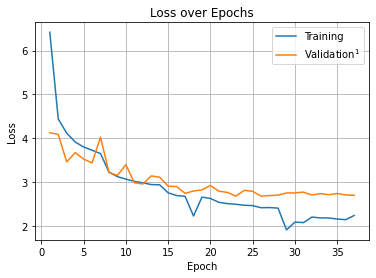
\includegraphics[scale=0.45]{flair_loss.png}
    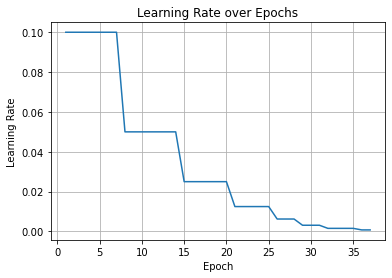
\includegraphics[scale=0.45]{flair_lrs.png}
    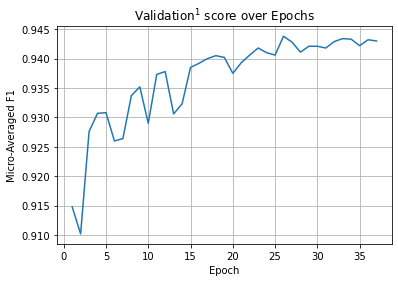
\includegraphics[scale=0.45]{flair_scores.png}
    \caption{Losess (up-left), learning rate (up-right) and $Validation^1$ scores (bottom) per epoch}
    \label{fig:flairtrain}
\end{figure}
\newpage
\section{BERT$^{NER}$}
\label{sec:app:bertner}
The tables below show the results of the models for each hyperparameter configuration on Validation$^2$ dataset. Table \ref{tab:bert_ner_no_scheduler} displays the results where the model was trained for 10 epochs and saved at the end of each. The Validation$^2$ results are obtained on specific epochs: 2, 3, 4, 6 and 10. 2, 3 and 4 are included as they were among the recommended hyperparameters. Epoch 6 and 10 are included as the former resulted in the highest Validation$^1$ ORG-F1 score while the latter was the last epoch. Table \ref{tab:bert_ner_scheduler} shows the results on Validation$^2$ dataset for the setting where a linear learning rate scheduler is used.

\begin{table}[h!]
    \centering
    \begin{tabular}{c| c c c| c c c}
    &\multicolumn{3}{c|}{Organization}&\multicolumn{3}{c}{Grant} \\
    Epoch&Precision&Recall&F1&Precision&Recall&F1\\
    \hline
    2     & 80.38	&84.14&82.22	&94.18&	96.95&95.55  \\
    3     & 78.76	&84.9&81.72	&94.51&	96.78&95.63  \\
    4     & 79.18	&84.18&81.6	&94.3&	96.89&95.58  \\
    6     & 79.88	&84.71&82.23	&94.73	&96.53&95.62  \\
    10   &  81.04	&80.24&80.64	&94.62&	96.38&95.49  \\
    \end{tabular}
    \caption{BERT$^{NER}$ results on Validation$^2$. Trained for 10 epochs without a scheduler, the model is saved after every epoch.}
    \label{tab:bert_ner_no_scheduler}
\end{table}


\begin{table}[h!]
    \centering
    \begin{tabular}{c| c c c| c c c}
    &\multicolumn{3}{c|}{Organization}&\multicolumn{3}{c}{Grant} \\
    Epoch&Precision&Recall&F1&Precision&Recall&F1\\
    \hline
    2     & 78.44&	85.8&	81.96&	94.59&	97.43&	95.99
 \\
    3     & 79.18&86.03&82.46&94.71&97.39&96.03
 \\
    4     & 79.41&85.88&82.52&94.95&97.38&96.15
 \\
    \end{tabular}
    \caption{BERT$^{NER}$ results on Validation$^2$. Trained for 2,3 and 4 epochs respectively with a scheduler, the model is saved after the training is done.}
    \label{tab:bert_ner_scheduler}
\end{table}

As the scores for Grant mentions are high in each setup, the model is chosen based on the scores on Organization mentions. Recall is favored over precision and based on this intuition, the model that is trained for 3 epochs with a learning rate scheduler is selected. This model has the highest recall for Organization mentions and the second highest F1 score. 


\section{Biencoder$_{ADPT}$}
\label{sec:app:biencoderadapt}
Table \ref{tab:biencoderadaptresapp} the scores of the models after each round on Training and Validation$^1$ splits for Biencoder$_{ADPT}$ with the second hyperparameter setting, the one where one round corresponds to two epochs and maximum number of tokens is set to 256 for the candidate representation.
\newpage

\vspace*{-3cm}\begin{table}[H]
    \centering
   \begin{tabular}{ccccc}
    &&&Micro-Averaged & Macro-Averaged\\
    Dataset & Round & Threshold     & Accuracy &Accuracy\\
    \hline
    Training & 1 & 0.5 & 62.36&64.44\\
    Training & 2 & 0.5 & 87.06&88.33\\
    Training & 3 & 0.5 & 90.3&91.09\\
    Training & 4 & 0.5 & 94.94&95.61\\
    \hline
    Training & 1 & 0.972&70.53&71.4 \\
    Training & 2 & 0.75 &91.66&92.29\\
    Training & 3 & 0.759&93.62&94.12 \\
    Training & 4 & 0.728&96.16&96.67 \\
    \hline
    Validation$^1$ & 1 & 0.5&63.62&70.03 \\
    Validation$^1$ & 2 & 0.5&82.56&87.07 \\
    Validation$^1$ & 3 & 0.5&84.16&88.21 \\
    Validation$^1$ & 4 & 0.5&86.26&89 \\
    \hline
    Validation$^1$ & 1 & 0.972&70.24&75.05\\
    Validation$^1$ & 2 & 0.75 &86.38&89.45\\
    Validation$^1$ & 3 & 0.759&86.74&89.94\\
    Validation$^1$ & 4 & 0.728&87.74&90.14\\
    \end{tabular}
    
    \vspace{0.5cm}\begin{tabular}{cccccc}
    &&&&EE Setting & \\
    Dataset & Round    & Threshold & Precision & Recall & F1-Score \\
    \hline
    Training & 1 & 0.5&100&0.02&0.04 \\
    Training & 2 & 0.5&96.68&57.56&72.16 \\
    Training & 3 & 0.5&99.13&67.77&80.5 \\
    Training & 4 & 0.5&99.16&87.66&93.06 \\
    \hline
    Training & 1 & 0.972&72.15&57.81&64.19 \\
    Training & 2 & 0.75&86.11&89.88&87.96 \\
    Training & 3 & 0.759&91.59&90.96&91.27 \\
    Training & 4 & 0.728 &95.85&96.45&96.15\\
    \hline
    Validation$^1$ & 1 & 0.5&0&0&0 \\
    Validation$^1$ & 2 & 0.5&83.75&42.69&56.55 \\
    Validation$^1$ & 3 & 0.5&87.22&44.76&59.16 \\
    Validation$^1$ & 4 & 0.5&83.84&60.3&70.15 \\
    \hline
    Validation$^1$ & 1 & 0.972 &66.03&55.7&60.43\\
    Validation$^1$ & 2 & 0.75  &69.64&79.98&74.45\\
    Validation$^1$ & 3 & 0.759 &72.9&73.99&73.44\\
    Validation$^1$ & 4 & 0.728 &74.81&77.91&76.33\\
    \end{tabular}
    
    \vspace{0.5cm}\begin{tabular}{cccccc}
    &&&&InKB Setting & \\
    Dataset & Round    & Threshold& Precision & Recall & F1-Score \\
        \hline
    Training & 1 & 0.5&62.36&76.58&68.74 \\
    Training & 2 & 0.5&85.86&93.79&89.65 \\
    Training & 3 & 0.5&89.02&95.44&92.12 \\
    Training & 4 & 0.5&94.11&96.6&95.34 \\
    \hline
    Training & 1 & 0.972&70.25&73.44&71.81 \\
    Training & 2 & 0.75 &93&92.07&92.53\\
    Training & 3 & 0.759&94.08&94.23&94.16 \\
    Training & 4 & 0.728&96.23&96.09&96.16 \\
    \hline
    Validation$^1$ & 1 & 0.5&63.62&75.26&68.95\\
    Validation$^1$ & 2 & 0.5&82.45&89.85&85.99\\
    Validation$^1$ & 3 & 0.5&83.89&91.37&87.47\\
    Validation$^1$ & 4 & 0.5&86.56&91.01&88.73\\
    \hline
    Validation$^1$ & 1 & 0.972&70.87&72.9&71.87 \\
    Validation$^1$ & 2 & 0.75 &90&87.56&88.76 \\
    Validation$^1$ & 3 & 0.759&89.32&89.07&89.2 \\
    Validation$^1$ & 4 & 0.728&90.22&89.53&89.87 \\
    \end{tabular}
    \caption{Intermediate Results for Biencoder$_{ADPT}$}
    \label{tab:biencoderadaptresapp}
\end{table}

\end{document}

